%%%%%%%%%%%%%%%%%%%%%%%%%%%%%%%%%%%%%%%%%%%%%%%%%%%%%%%%%%%%%%%%%%%
\chapter{Design and Implementation} \label{chap:design-impl}
The module for an alert prediction is named Hawkular Data Mining. Source code is versioned in Git and
hosted on Github\footnote{Available at \url{https://github.com/hawkular/hawkular-datamining}.} under
license Apache version 2.0.

The project is split into several Maven artifacts. This approach decomposes problem into smaller parts
which have dedicated functionality and can be easy reused in other projects. It also ensures that
third party dependencies are loaded only for certain artifacts, where are needed.

Figure \ref{appen:maven-deps} shows dependency tree of \texttt{datamining-dist}, which is the top level artifact.
The most important modules are listed in Table \ref{tab:datamining-modules}. All ids of the listed artifacts have prefix
\texttt{hawkular-datamining}.

\begin{table}[h]
    \begin{center}
        \begin{tabular}{l|l}
            \textbf{Artifact Id} & \textbf{Description} \\ \hline \hline
            \texttt{parent} & Manages shared dependencies and versions. \\
            \texttt{forecast} & Core library for time series modeling and forecasting. \\
            \texttt{api} & API used within Data Mining. \\
            \texttt{cdi} & Support for context dependency injection. \\
            \texttt{rest} & Web archive for standalone usage without Hawkular. \\
            \texttt{dist} & Web archive with Hawkular integration code. \\
            \texttt{itest} & Artifact for integration tests.
        \end{tabular}
        \caption{Hawkular Data Mining modules.}
        \label{tab:datamining-modules}
    \end{center}
\end{table}

In the following sections the most important parts of the implementation are described. This text focuses on
design of data structures, interaction between them and algorithms.

    %%%%%%%%
    \section{Forecast Package}
    The forecast package is time series modelling and forecasting library. It contains several time series models
    and utility classes for time series modelling. It is designed to be easy used in any Java project. The footprint
    of the artifact is small. It depends only on Apache Math, Commons, Guava and Jboss logging.

    The core data structures from \texttt{datamining-forecast} package are interfaces of time series models
    and forecasters. Some of the methods are listed in Algorithm \ref{alg:models}. These two interfaces are related but
    not the same. Each time series model should be capable of predicting and learning. Models also collect
    initialization and running statistics so it is possible to make assumptions of the forecasting accuracy.

    The main difference between forecaster and time series model is that forecaster is designed for online learning
    and it autonomously selects the most appropriate time series model. Time series models by default are not
    designed for online learning, however it can be accomplished with a wrapper class.

    Metric in the Data Mining is represented as structure \texttt{MetricContex} which contains metadata like
    collection interval, metric id and tenant id. Collection interval is necessary for calculating timestamps of
    predicted points.

    \begin{lstlisting}[caption={Interface for time series models.}, language=Java, label={alg:models}]
interface TimeSeriesModel {
    void learn(List<DataPoint> ts);
    List<DataPoint> forecast(int steps);
    int numberOfParameters();
    MetricContext context();
    AccuracyStatistics initStatistics();
    AccuracyStatistics runStatistics();
    ...
     }
    \end{lstlisting}

    List of implemented models, statistical and utility classes for time series manipulation:

    \begin{multicols}{2}
        \begin{itemize}
            \item Simple ex. smoothing
            \item Double ex. smoothing
            \item Triple ex. smoothing
            \item Weighted moving average
            \item Automatic forecaster
            \item Augmented Dickey\,--\,Fuller test
            \item Time series decomposition
            \item Autocorrelation function
            \item Time series lagging
            \item Time series differencing
            \item Automatic period identification
        \end{itemize}
    \end{multicols}

        %%%%%%%%
        \subsection{Automatic Forecaster}
        One of the most important forecasting classes in Data Mining is \\\texttt{AutomaticForecaster}. This class
        autonomously decides which time series model should be used for modelled time series. Currently it decides from
        three implemented models: simple, double and triple exponential smoothing. Other models which implement
        interface \\\texttt{TimeSeriesModel} can be easily added.

        Most importantly, this class is capable of dealing with concept drift. It holds circular buffer of historical
        metrics and if statistical properties of the underlying time series changes content of the buffer is used for
        selecting new model.

        The strategy when a new model should be selected is configurable. The system currently
        supports two strategies. The first strategy selects new model periodically each $n$ observations.
        The second one is more sophisticated and it selects a new model only when the error produced on learning data
        exceeds by $x\%$ error calculated on learning points when model was initialized.

        Model selection is based on information criterion from Section \ref{sec:model-quality}. Automatic forecaster in
        successive steps calls optimizers of given models and then selects the best with the lowest information
        criterion. Used criterion is configurable for each forecaster.

        %%%%%%%%
        \subsection{Model Optimizers}
        Model optimizers are the most important part of the models implementation. If the model parameters are not
        estimated correctly, model produces high forecasting error.

        The idea behind optimization is to find such
        parameters that describe training data the best \cite{hyndman-state-space}. Optimization criterion can be: mean
        squared error, mean absolute error and likelihood. These criterion basically computes errors produced by ahead
        predictions. The number of prediction steps depends on the forecaster's objective. The most common is to use
        only one step ahead. Data Mining currently supports only MSE criterion but others can be easy added.

        The criterion is returned from model's objective function. This objective function is then passed to non-linear
        optimization algorithm from Apache Math Commons. This library implements several optimization algorithms:
        Nelder-Mead simplex, multi-directional simplex and bound optimization by quadratic approximation (BOBYQA).
        These algorithms do not need computed derivatives of the cost function.

        In terms of the lowest execution time and quality of the estimated parameters the best results were produced by
        Nelder-Mead simplex algorithm.

        Table \ref{tab:open-forecast-perf} contains comparison of optimizers execution times from \texttt{OpenForecast}
        and R implementation. This section adds execution time of Data Mining implementation. Complete execution times
        are listed in Table \ref{tab:datamining-perf}. Execution times of Data Mining's optimizers are in some
        cases faster than R. Quality of the produced forecasts is discussed in Chapter \ref{chap:evaluation}.

        \begin{table}[h]
            \begin{center}
                \begin{tabular}{l|c|c|c}
                    \textbf{Model} & \textbf{OpenForecast} & \textbf{R \texttt{forecast}} &
                        \textbf{Data Mining}\\ \hline \hline
                    Simple ex. & 4.91 sec. & 0.003 sec. & 0.033 sec.\\
                    Double ex. & 9.31 sec. & 0.006 sec. & 0.002 sec. \\
                    Triple ex. & 6.45 sec. & 0.209 sec. & 0.023 sec. \\
                \end{tabular}
                \caption{Execution time of parameters estimation for exponential smoothing models.}
                \label{tab:datamining-perf}
            \end{center}
        \end{table}

    %%%%%%%%
    \section{API Package}
    The next package is \texttt{api}. It depends on \texttt{forecast} and it eventually could
    depend on another library for data analysis, for instance a library for an outlier detection. In this package there
    is a code necessary for using Data Mining as application which analyzes multiple metrics, for example classes for
    accessing data analysis objects for given metric.

    The interface \texttt{SubscriptionManager} was designed for accessing time series analysis objects. Some of its
    methods are listed in Algorithm \ref{alg:sub-manager}. Implementation of this interface could store entities in
    database. However, Data Mining directly does not use any database. Therefore \\ \texttt{SubscriptionManager}
    holds all objects in memory. Internally it stores objects in a map where the key is tenant and value another
    map where the key is metric id and value the object for data analysis\,--\,\texttt{Subscription}.

    \begin{lstlisting}[caption={Interface \texttt{SubscriptionManager}.}, language=Java, label={alg:sub-manager}]
interface SubscriptionManager {
     void subscribe(Subscription, Owner);
     void unsubscribe(tenant, metric, Owner);
     Subscription model(tenant, metric);
     ...
     }
    \end{lstlisting}

    For subscribing it is necessary to specify the owner of the prediction configuration. It was specially added for
    integration with Inventory. It is more described in Section \ref{sec:dist}.

    Object \texttt{Subscription} holds instance of \texttt{AutomaticForecaster} and it could also hold another
    data analysis objects. Its role is to delegate calls to the business logic objects.

    Class diagram of the most important classes from \texttt{forecast} and \texttt{api} is depicted in Appendix
    \ref{appen:class-diagram}.

    Some of the service classes like \texttt{SubscriptionManager} are used in several other classes and also multiple
    implementation could exist (in memory or database implementation). Therefore dependency injection
    design pattern was introduced. Used technology is Java context dependency injection (CDI). In order to keep
    API classes clean module \texttt{cdi} with CDI configuration was introduced. It directly depends on \texttt{api},
    but does not add any other business logic.

    %%%%%%%%
    \section{REST Package}
    Package \texttt{rest} contains implementation of REST services provided by Data Mining. Implementation is
    compatible with standard JAX-RS.

    Data Mining REST API is designed to operate on the forecasting engine. When the module is deployed into Hawkular
    main interaction with Data Mining goes through Inventory REST API and metric data are collected from JMS topic.
    However, this is not limited and Data Mining offers alternative REST endpoints which can be used for
    example in standalone deployment.

    REST API provides following capabilities:

    \begin{itemize}
        \item Operate on subscriptions\,--\,enable and disable prediction.
        \item Push learning data to the engine.
        \item Get predictions for any number of steps ahead.
        \item Configure automatic forecaster.
        \item Get information about model being used and statistics of the predictions.
    \end{itemize}

    Accurate and more comprehensive REST API documentation is available on Hawkular web page\footnote{Available at
    \url{http://www.hawkular.org/}.}. This documentation is automatically generated using Swagger framework.

    %%%%%%%%
    \section{Distribution Package\,--\,Integration into Hawkular} \label{sec:dist}
    As it was mentioned before, the build produces two web archives, one for standalone usage and another for
    deployment into Hawkular. The second web archive adds extra functionality for interacting with the other Hawkular
    components.

    In Hawkular all entities are stored in Inventory, therefore Data Mining uses this module
    for querying metric definitions and it adds some extra attributes necessary for predictions. Another module
    which is used by Data Mining is Hawkular Metrics. Diagram \ref{img:hawkular-interaction} shows Data Mining
    integration into Hawkular.

    \begin{figure}[H]
        \begin{center}
            \scalebox{0.32}{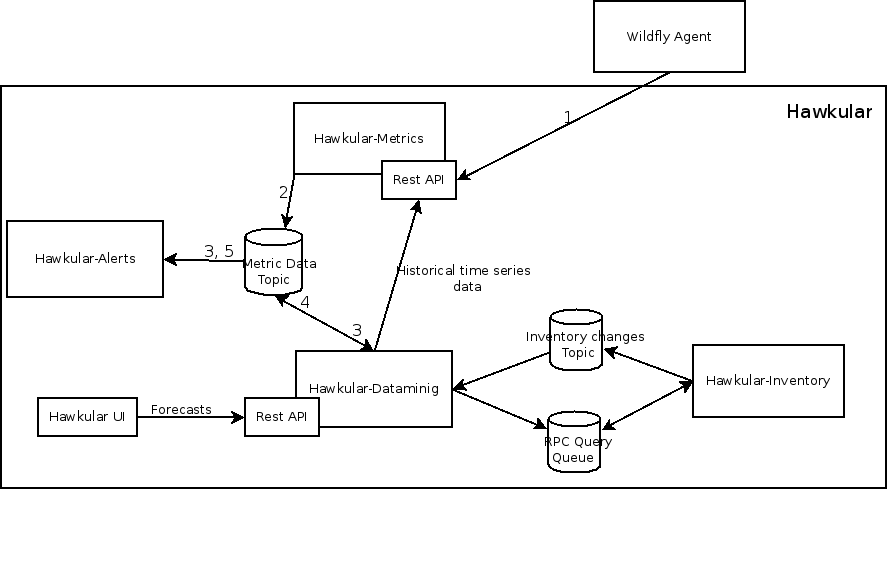
\includegraphics{img/src/architecture.pdf}}
            \caption{The integration into Hawkular.}
            \label{img:hawkular-interaction}
        \end{center}
    \end{figure}

    When Data Mining is deployed into Hawkular, users can enable predictions by creating Relationship\footnote{Entity
    from Inventory which can be created between arbitrary two entities.} from tenant to the target entity. Target
    entity can be metric, metric type or tenant. When relationship is created from tenant to tenant, predictions are
    enabled for all metrics under given tenant. Similarly, when a target entity is a metric type, predictions are
    enabled for all metrics of that type. In Figure \ref{img:relationship} is depicted part of the structure of
    inventory with enabled predictions.

    Relationships also store properties needed for predictions. One of them is forecasting horizon which tells how
    many prediction steps are performed for each incoming metric data point. With this approach of storing
    relationships in Inventory, Data Mining does not have to use any database for entities related to predictions.
    This approach was achieved without any changes to Inventory data model, this shows that Inventory's generic data
    model build on top of graph database\footnote{Compatible with Apache Tinkerpop.} is good approach for storing data
    model in this domain.

    \begin{figure}[H]
        \begin{center}
            \scalebox{0.35}{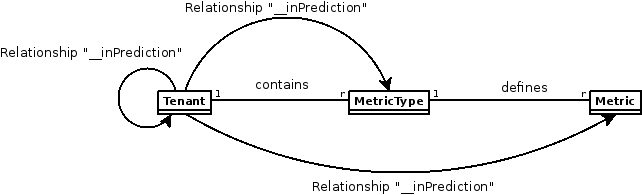
\includegraphics{img/src/inventory.pdf}}
            \caption{Relationship between entities of Inventory.}
            \label{img:relationship}
        \end{center}
    \end{figure}

    Any changes in Inventory are propagated to Data Mining by subscribing to specific events. This propagation is done
    through JMS topic where Inventory sends these events. However, on application start Data Mining also needs to query
    all predictive relationships from Inventory. For this purpose JMS request-response communication was implemented in
    Inventory. Any component which has access to internal messaging subsystem can construct a query and send it for
    execution to Inventory. REST API approach was also proposed but it could expose vulnerability\,--\,client
    could access any data objects of any tenant. Diagram \ref{img:sequence-enab-pred} depicts sequence of calls
    when prediction gets enabled.

    \begin{figure}[H]
        \begin{center}
            \scalebox{0.30}[0.20]{\includegraphics[angle=0]{img/src/uml-enable-predictions-sequence.pdf}}
            \caption{Sequence diagram of enabling predictions.}
            \label{img:sequence-enab-pred}
        \end{center}
    \end{figure}

    From Diagram \ref{img:sequence-enab-pred} it is clear that when a prediction gets enabled, historical metrics
    are queried from Metrics module. This means that Data Mining needs to access metrics of all tenants. It is
    similar scenario to getting all predictive relationships from Inventory. It could not be implemented via REST API
    because of potential vulnerability and JMS based query was rejected by Metrics developers.

    Another two solutions were proposed. The first was to bypass Metrics and query data directly from Cassandra.
    The second was to inject Metrics as CDI bean and directly use its Java API. The first solution was refused because
    the schema is maintained by Metrics and it can eventually change and also the backed database (Cassandra) can
    change. The final and implemented solution injectings Metrics as CDI bean. This approach assumes that Metrics
    are deployed in the same application server as Data Mining. From the performance perspective it is faster that
    JMS or REST calls.

    Diagram \ref{img:sequence-incoming-data} shows complete data flow from agent to alerts evaluation engine.
    First metric data is sent by agent to Metrics where it is stored to database. Then it is sent to JMS topic
    and consumed by Alerts and Data Mining. In parallel Alerts evaluates alerts criteria and Data Mining computes
    predictions. After computation the predicted data are sent back to the same JMS topic and consumed by Alerts.
    At this point an alert of predicted metrics can be triggered.

    Data Mining changes \texttt{id} of predicted points in order to be able to distinguish original time series from
    predicted. For predicted metrics Alerts can evaluate the same conditions as for original time series or use
    different ones, more in Section \ref{sec:alerts-conditions}.

    \begin{figure}[H]
        \begin{center}
            \scalebox{0.33}[0.24]{\includegraphics[angle=0]{img/src/uml-incoming-data-sequence.pdf}}
            \caption{Sequence diagram of incoming data from agent.}
            \label{img:sequence-incoming-data}
        \end{center}
    \end{figure}

        %%%%%%%%
        \subsection{Alerts and Conditions} \label{sec:alerts-conditions}
        In this section it is briefly described how the alerting system works. Alerts is a separate module
        which is responsible for firing alerts based on defined conditions. As it is depicted in Diagram
        \ref{img:sequence-incoming-data} Alerts listens to the JMS topic and if conditions for given metric are
        positively evaluated an alert is fired.

        Alerts data model is little bit more complicated though, as for each unique metric id multiple conditions can be
        defined. These conditions are evaluated for every received metric data point on the bus. Conditions are
        grouped under a trigger. If the result of evaluation is possitive than the tigger triggers an action. This
        action can be for instance sending an email, sms or perform a webhook\dots

        Triggers can be grouped which facilitates creation of the similar triggers. Particulary this can be used for
        creating triggers for predictive metrics. If there is a trigger defined for the original metric it can be
        duplicated and used for predicted metrics.

        If necessary the conditions can be changed in
        order to not trigger an alert if the predictions are not very accurate. Trigger dampening can be used for this.
        So for the trigger which operates on predicted metrics dampening can be set as follows: \emph{``fire an alert if
        $X$ consecutive evaluations of conditions are positive``}.

        %%%%%%%%
        \subsection{Hawkular UI}
        Predictive charts in Hawkular are located in Metric explorer tab. In Figure \ref{img:hawkular-explorer}
        predictive chart for metric accumulated garbage collection duration is shown. In this case automatic
        forecaster decided to use seasonal model of some automatically identified period. Note that for displaying
        original time series in the chart buckets were used, so the periods would be more easily seen on raw data
        points.

        \begin{figure}[H]
            \begin{center}
%                \scalebox{0.33}[0.24]{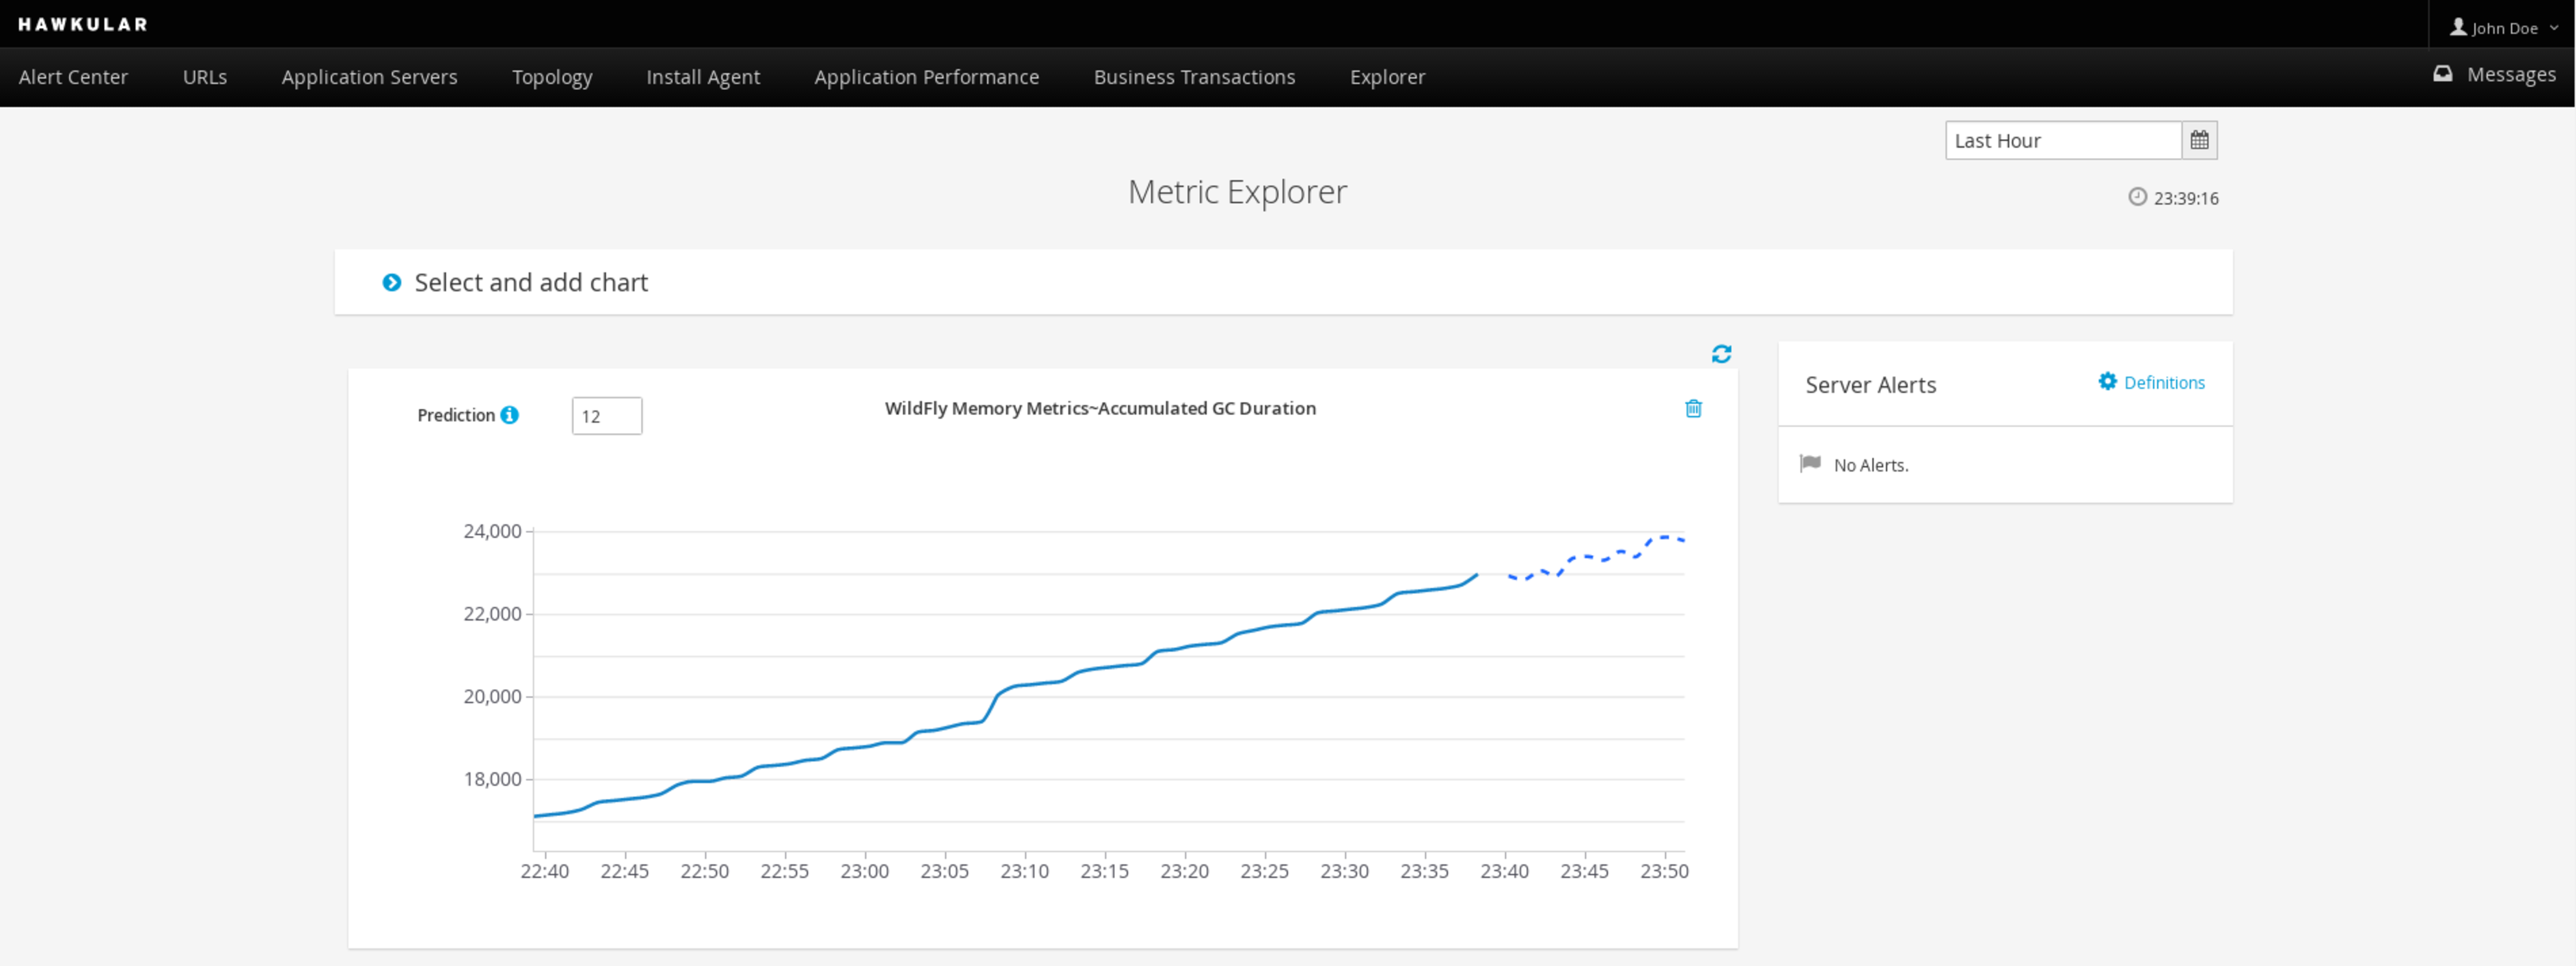
\includegraphics[angle=0]{img/hawkular-explorer.pdf}}
                \scalebox{0.185}[0.28]{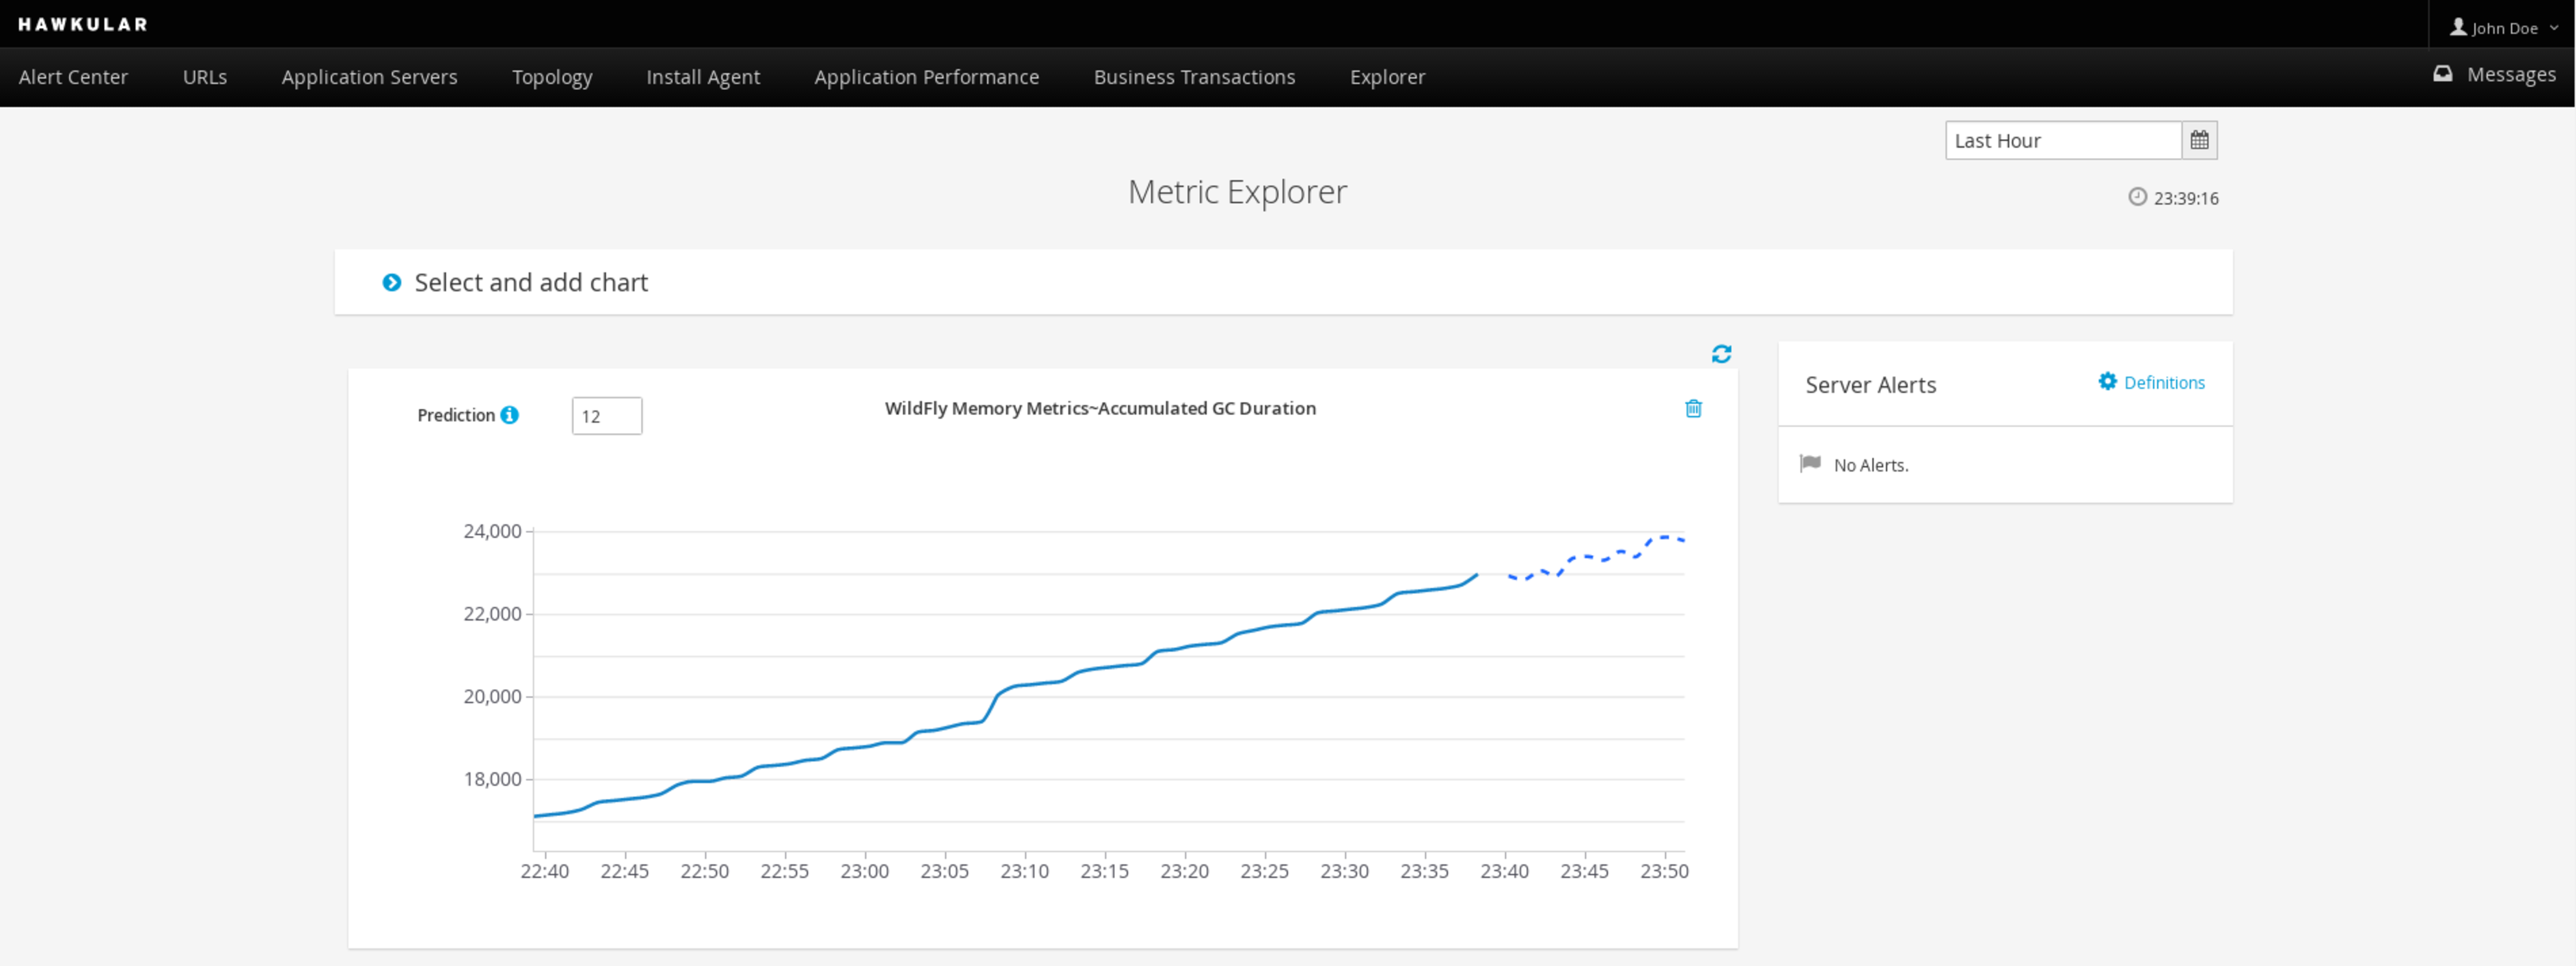
\includegraphics[angle=0]{img/hawkular-explorer.pdf}}
                \caption{Metric explorer tab in Hawkular user interface.}
                \label{img:hawkular-explorer}
            \end{center}
        \end{figure}

        After adding concrete chart predictions can be enabled by increasing prediction horizon input.
        So there is no need to enable predictions manually by creating relationship in Inventory.

        Predictive charts were used from repository \texttt{hawkular-charts}. These charts are built on top of
        D3\footnote{Avalilable at \url{https://d3js.org/}.} library and encapsulated as Angular directives.

    %%%%%%%%
    \section{Test Automation and Documentation}
    Core functionality of the application is covered by unit tests. Junit framework is used for this type of tests.
    Because Data Mining interacts with other applications and modules, integration tests are also implemented. These
    tests are executed from Maven profile which starts web server with necessary modules deployed.

    The last type of implemented tests are end-to-end tests which call REST endpoint of one module and expect result
    in call from another module. These types of tests are also executed in Maven profile with running web server.
    End-to-end tests for Data Mining project live in the main Hawkular integration repository\footnote{
    Available at \url{https://github.com/hawkular/hawkular}.}.

    All tests are automatically executed every time developer creates a pull request or pushes code to the master
    branch. For this Travis continuous integration platform was used, which is available for free for open source
    projects on Github.

    Documentation is directly written in Java code as javadoc. REST API documentation is also directly
    written in source code using Swagger framework and automatically generated at build time
    \footnote{Available at \url{http://www.hawkular.org/docs/rest/rest-datamining.html}.}.

    %%%%%%%%
    \section{Releases}
    At the time of writing this thesis, there was only one release with version \texttt{0.1.Final}. It is also available
    in the Maven central repository. Complete group id is \texttt{org.hawkular.datamining}. The most important
    artifact ids are listed in Table \ref{tab:datamining-modules}. Release notes are available on
    Github\footnote{Available at \url{https://github.com/hawkular/hawkular-datamining/releases}.}.

    %%%%%%%%
    \section{Retrospective}
    In this section it is mentioned how the project was changing during the implementation, what did not worked well and
    what could have been done better.

    At the beginning of the project Apache Spark\footnote{Open source cluster computing framework available at
    \url{https://spark.apache.org/}.} was used for building regression models. Its machine learning library (MLIB)
    offers several learning algorithms. In Data Mining linear regression with stochastic gradient descent was used.
    Because the gradient is stochastic, produced predictions are not very robust and quickly change by significant
    value.

    Spark was mainly used because of its streaming extension that can handle
    high-throughput stream data \cite{apache-spark}. There is also time series library
    \texttt{spark-ts}\footnote{Available at \url{https://github.com/sryza/spark-timeseries}.} which contains some
    time series models but does not offer functionality of automatic model selection.

    Due to the problems with linear regression discussed in Section \ref{sec:linear-regression} and lack of automatic
    forecaster, decision was made to drop Spark and directly implement exponential smoothing models.

    During the implementation a lot of time was spent on integration with other modules, with Inventory in particular.
    The problem was that Inventory is developed by another party and any concrete document
    describing the integration was not proposed. The design of the integration was understood differently
    by both parties, which lead to reimplementing of some parts. Therefore it is better to precisely define the
    integration interface with other modules or projects.

%%%%%%%%%%%%%%%%%%%%%%%%%%%%%%%%%%%%%%%%%%%%%%%%%%%%%%%%%%%%%%%%%%%
\chapter{Evaluation of Implemented Models} \label{chap:evaluation}
Evaluation process compares predictive capabilities of the implemented models to statistics produced by similar models
from R language. Models from R language are selected because they are widely used by forecasters all around the
world and de facto standard for statistical science \cite{kleiber2008applied}, therefore, for this work considered
as referential.

To be specific used models are from package
\texttt{forecast}\footnote{Available at \url{https://cran.r-project.org/web/packages/forecast/index.html}.}.
Function used for fitting models is \texttt{ets}. This function accepts several configuration parameters for instance:
what model should be used, statistics for objective function, information criterion\dots For testing in this work model
parameter is set to \texttt{ANN}, \texttt{AAN} and \texttt{AAA} for simple, double and triple exponential smoothing,
objective statistics for minimization is MSE and parameter damped set to false.

The used methodology and more comprehensive description of tested objectives is listed in Section \ref{sec:methodology}.

    %%%%%%%%
    \section{Methodology} \label{sec:methodology}
    In order to evaluate forecasting quality of the implemented models it is necessary to use well defined
    methodology with test data which contains broad range of patterns: white noise, monotonicity, random
    shocks, trend and seasonality.

    Most importantly methodology should not evaluate forecasting accuracy how well model
    fits the historical data. Instead it should evaluate forecast accuracy using genuine forecasts\,--\,test
    how well model performs on new data \cite{otexts}. Therefore it is necessary to split time series into training
    and test set.

    The size of the test set is usually 20\% of the total sample. Albeit the size of test set depends on how
    long all the sample is and how far ahead one wants to forecast.

    Outline of the methodology used in this work:
    \begin{enumerate} \label{enum:methodology}
        \item Divide data sample into training and test set.
        \item Set $k = size(trainingSet)$.
        \item Train model on the training set. And learn up to $k^{th}$ observation. \label{item:train}
        \item Compute n-step ahead forecast $\hat{y}$ and error $\epsilon = y-\hat{y}$.
        \item Set $k = k+1$ and continue at step \ref{item:train} until $k=size(trainingSet + testSet)$.
        \item Calculate MSE of produced errors.
    \end{enumerate}

    As it was described earlier time series used for testing should contain one or even combine more patterns together.
    Test samples used in this work are depicted in Appendix \ref{appen:testing-samples}. Each sample contains white
    noise, random shocks and one or more of the following patterns: monotonicity, trend and seasonality. Names and
    description of test samples are listed in Table \ref{tab:test-samples-description}.

    \begin{table}[h]
        \begin{center}
            \begin{tabular}{l|l}
                \textbf{Time Series Name} &  \textbf{Description} \\ \hline \hline
                \texttt{wn} & Constant white noise. \\
                \texttt{trendUpLow} & Upward trend with white noise. \\
                \texttt{trendDownHigh} & Downward trend of high variance. \\
                \texttt{sine} & Constant sine with white nosie. \\
                \texttt{sineTrend} & Sine with trend and white noise. \\
            \end{tabular}
            \caption{Description of test samples.}
            \label{tab:test-samples-description}
        \end{center}
    \end{table}

    The last part what figures in our methodology is training size. Let's say that one would like to forecast one hour
    ahead and Wildfly Agent collects most of the metrics in five minute intervals. Thus forecasting horizon of one
    hour corespondes to 12 observations and training set should be at least long 48 observations.

    Interesting is also to find out if forecasting accuracy changes for larger training set. Therefore it
    was decided to add training sets of length 100 and 200 observations.

    In the following sections each model is tested using methodology from Section \ref{enum:methodology} on
    samples from Table \ref{tab:test-samples-description} of training size of 48, 100 and 200 observations with
    forecasting horizon set to: 1, 6 and 12 steps ahead. The size of test set is always 12 observations.

    Following notation is used to identify test cases:
    \begin{itemize}
        \item \emph{trainSampleSize\,--\,testSampleSize (forecastingHorizon)}
    \end{itemize}
    So for instance 48\,--\,12(1) denotes: training sample of size 48 observations, 12 test observations and
    forecasting horizon 1 step ahead.

    %%%%%%%%
    \section{Results}
    Complete test results are listed in Appendix \ref{appen:chap:results}. The top value in each cell is the result
    from R and below is the result from Data Mining. All measured values are in mean squared error. The table contains
    lot of data, however this work focuses on answering these two questions:

    \begin{enumerate}
        \item \emph{How well do the Data Mining models perform compared to R models?} \label{itm:question2}
        \item \emph{Does the size of training set affect quality of the forecasts?} \label{itm:question1}
    \end{enumerate}

    The first question can be answered by calculating ratios of Data Mining MSE to R MSE. If the ratio is lower than
    one it means that Data Mining model forecast more accurately.

    From the test results it can be shown how many tests cases have lower ratio or even better it is to split ratios
    into following intervals:
    lower than 1, \interval[{1,1.01}], \interval[{1.01,1.05}], \interval[{1.05,1.10}], \interval[{1.1,1.2}]
    and higher than 1.2. More aggregated representation is to calculate averages of these ratios for each test case.

    In order to get the answer for the second question it is necessary to compare MSE statistics produced by Data
    Mining models. For instance compare the result of test case 48\,--\,12(1) on \texttt{wn} sample to the same test
    case but with longer training set and analogously for other test samples and longer forecasting horizons. With
    this approach there would be too many results to compare. So this work first calculates averages of mean squared
    error of each test case, so the average for 48\,--\,12(1) is the average of all test samples (\texttt{wn},
    \texttt{trendUpLow}\dots) \\ of given test case.

    Chart with clear results is constructed for each of these two questions. The results of these charts are
    described in the following sections.

        %%%%%%%%
        \subsection{Simple Exponential Smoothing} \label{sec:results-simple}
        Raw results for simple exponential smoothing are listed in Table \ref{appen:tab:simple-results}.
        Pie Chart \ref{img:results-simple-pie} shows that Data Mining simple exponential smoothing model produces
        lower MSE than R in 38\% of all forty-five test cases and 38\% tests results are equal or worse at mosts than
        1\%. The test with worst result has 8\% higher MSE than equivalent R model.

        Data Mining's best result has 23\% lower MSE than the result from R model. It is for test case 100\,--\,12(1)
        on test sample \texttt{trendUpLow}.

        \begin{figure}[H]
            \begin{center}
                \begin{tikzpicture}
                    \pie[text=legend, radius=2, color={green!100 , green!100, green!80, green!50, yellow!60}]
                    {38/<1,
                    16/=1,
                    22/\interval[{1,1.01}],
                    18/\interval[{1.01,1.05}],
                    7/\interval[{1.05,1.10}]}
%                    0/ \interval[{1.1,1.2}],
%                    0/ >1.2}
                \end{tikzpicture}
                \caption{The proportion of Data Mining MSE to R MSE ratios split into intervals.}
                \label{img:results-simple-pie}
            \end{center}
        \end{figure}

        Chart \ref{img:results-simple-r} shows average ratios of Data Mining MSE to R MSE for each test case. These
        results are finer variants of results from Chart \ref{img:results-simple-pie}. It highlights that only three
        test cases out of nine have in average higher MSE than R and at most 2\% higher. It also shows that for
        larger training set Data Mining simple exponential smoothing in average produces lower MSE than R and
        on shorter training set R produces lower MSE than Data Mining.

        \begin{figure}[H]
            \begin{center}
                \scalebox{0.65}[0.5]{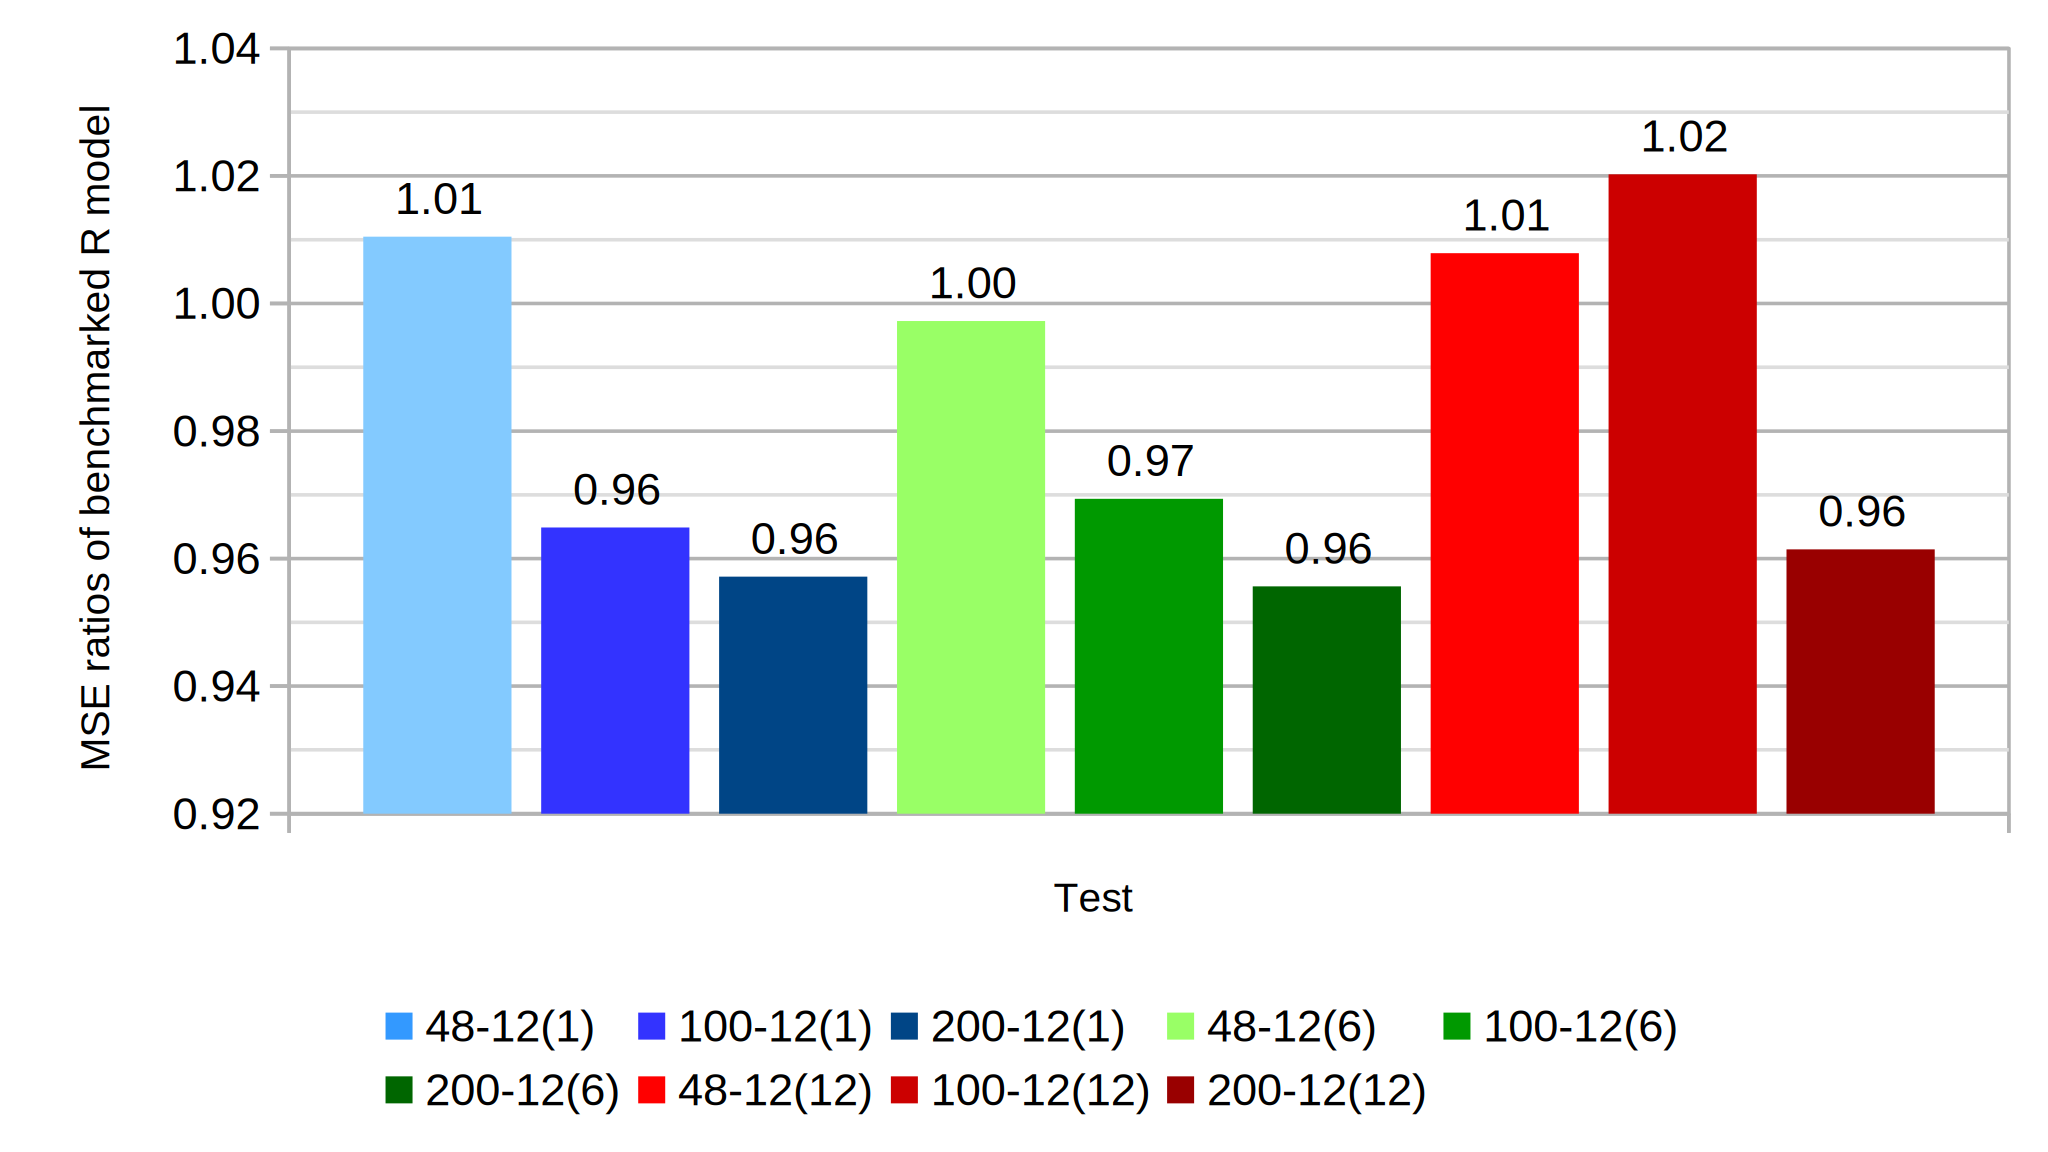
\includegraphics[angle=0]{img/src/results-simple-r.pdf}}
                \caption{Test results for triple exponential smoothing. Comparison to reference R model.}
                \label{img:results-simple-r}
            \end{center}
        \end{figure}

        Averages for each test case of Data Mining MSE are listed in Chart \ref{img:results-simple-mse}. This chart
        shows that the lowest average MSE are produced in test cases with training size of 48 observations. Therefore
        for simple exponential smoothing it is not necessary to use longer training set in order to get lower prediction
        error. Note that training samples contains randomly generated shocks. Therefore if more shocks are located later
        in time series than test cases for larger training sample can have higher MSE.

        \begin{figure}[H]
            \begin{center}
                % width, height
                \scalebox{0.65}[0.5]{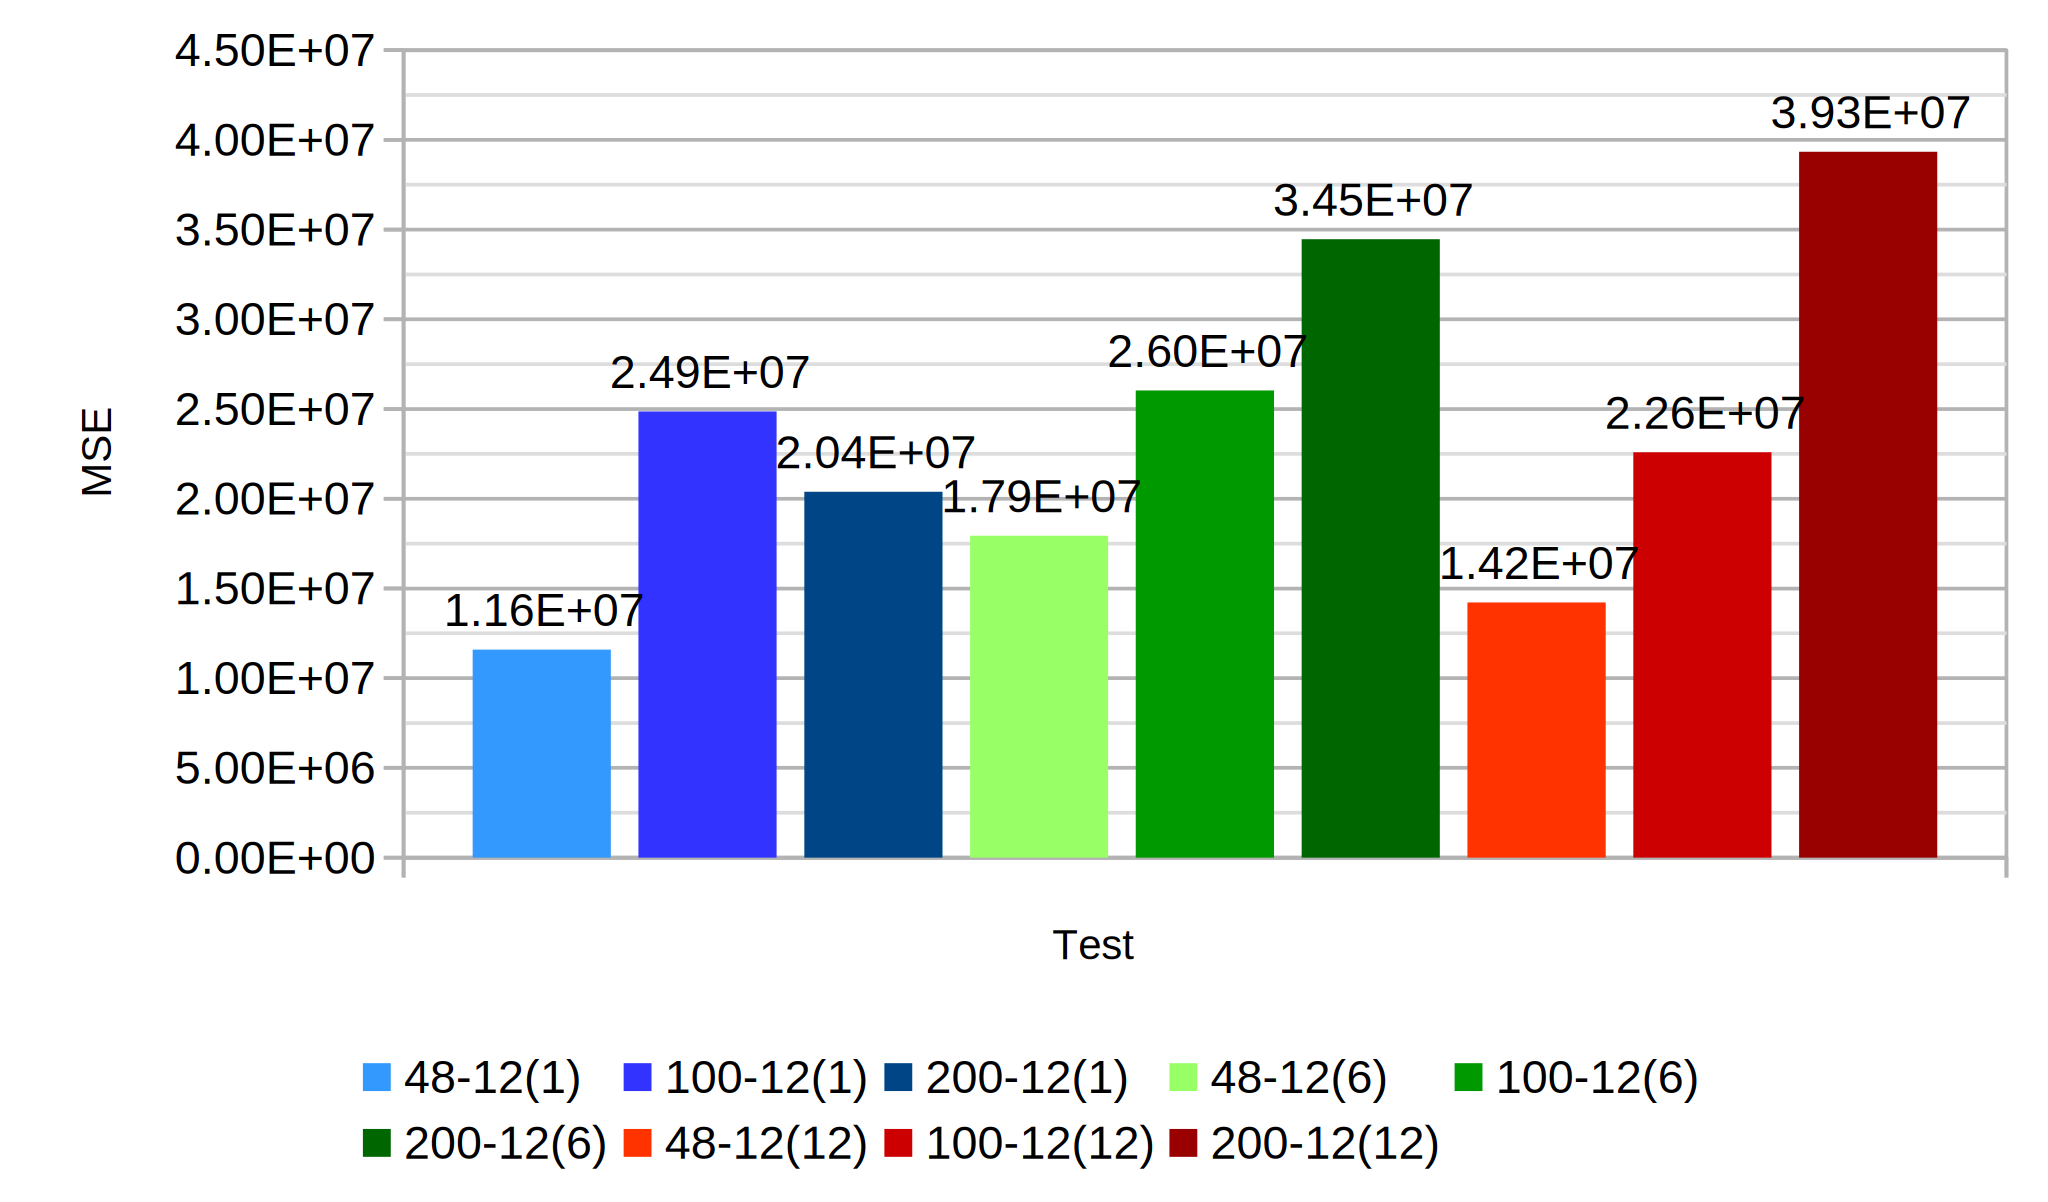
\includegraphics[angle=0]{img/src/results-simple-mse.pdf}}
                \caption{Test results for simple exponential smoothing. Average values of MSE for all tests samples.}
                \label{img:results-simple-mse}
            \end{center}
        \end{figure}

        %%%%%%%%
        \subsection{Double Exponential Smoothing} \label{sec:results-double}
        Complete raw tests results for double exponential smoothing are listed in Table \ref{appen:tab:double-results}.
        Chart \ref{img:results-double-pie} emphasizes that in 51\% tests Data Mining produces lower MSE than the
        equivalent R model. Five tests fall into the interval \interval[{1.1,1.2}] and one test has higher
        MSE than 20\%. Best result is for test case 100\,--\,12(12) where Data Mining produces lower MSE of 13\%.

        Averages of MSE ratios are depicted in Chart \ref{img:results-double-r}. Only three test cases have higher
        MSE than 1\% to maximum 6\%. The chart also shows that in average the
        lowest MSE ratios are for training set of length 48 observations. It meas that if results are compared to
        R in terms of training size R produces higher mean square error for larger training sets.

        \begin{figure}[H]
            \begin{center}
                \begin{tikzpicture}
                    \pie[text=legend, radius=2, color={green!100 , green!50, yellow!50, red!60, red!80}]
                    {51/<1,
                    27/\interval[{1.01,1.05}],
                    9/\interval[{1.05,1.10}],
                    11/\interval[{1.1,1.2}],
                    2/>1.2}
                \end{tikzpicture}
                \caption{The proportion of Data Mining MSE to R MSE ratios split into intervals.}
                \label{img:results-double-pie}
            \end{center}
        \end{figure}

        \begin{figure}[H]
            \begin{center}
                \scalebox{0.65}[0.5]{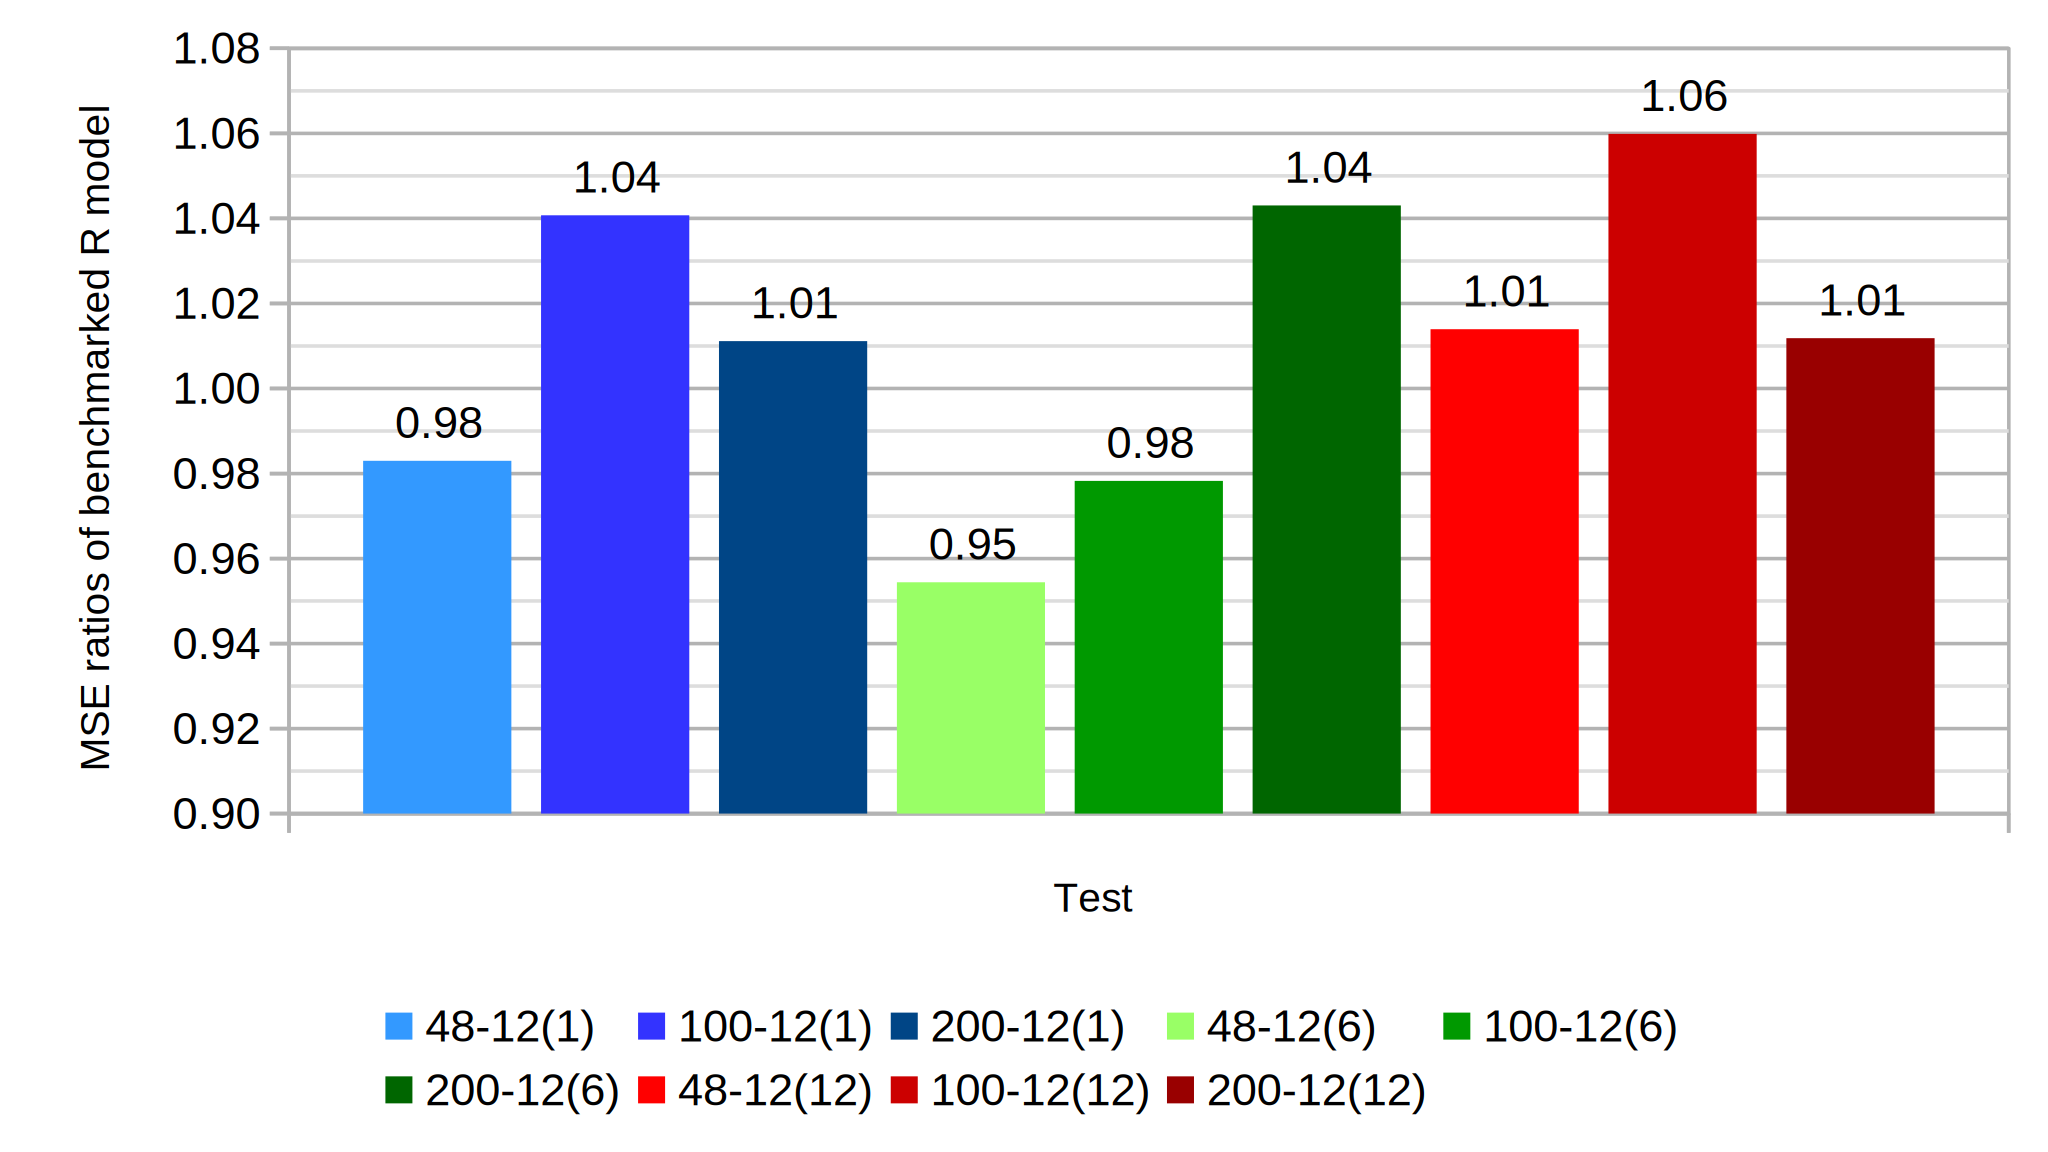
\includegraphics[angle=0]{img/src/results-double-r.pdf}}
                \caption{Test results for double exponential smoothing. Comparison to reference R model.}
                \label{img:results-double-r}
            \end{center}
        \end{figure}

        The last chart for double exponential smoothing is \ref{img:results-double-mse}.
        It shows that model similarly as simple exponential smoothing produces higher MSE for larger training sets.

        \begin{figure}[H]
            \begin{center}
                \scalebox{0.65}[0.5]{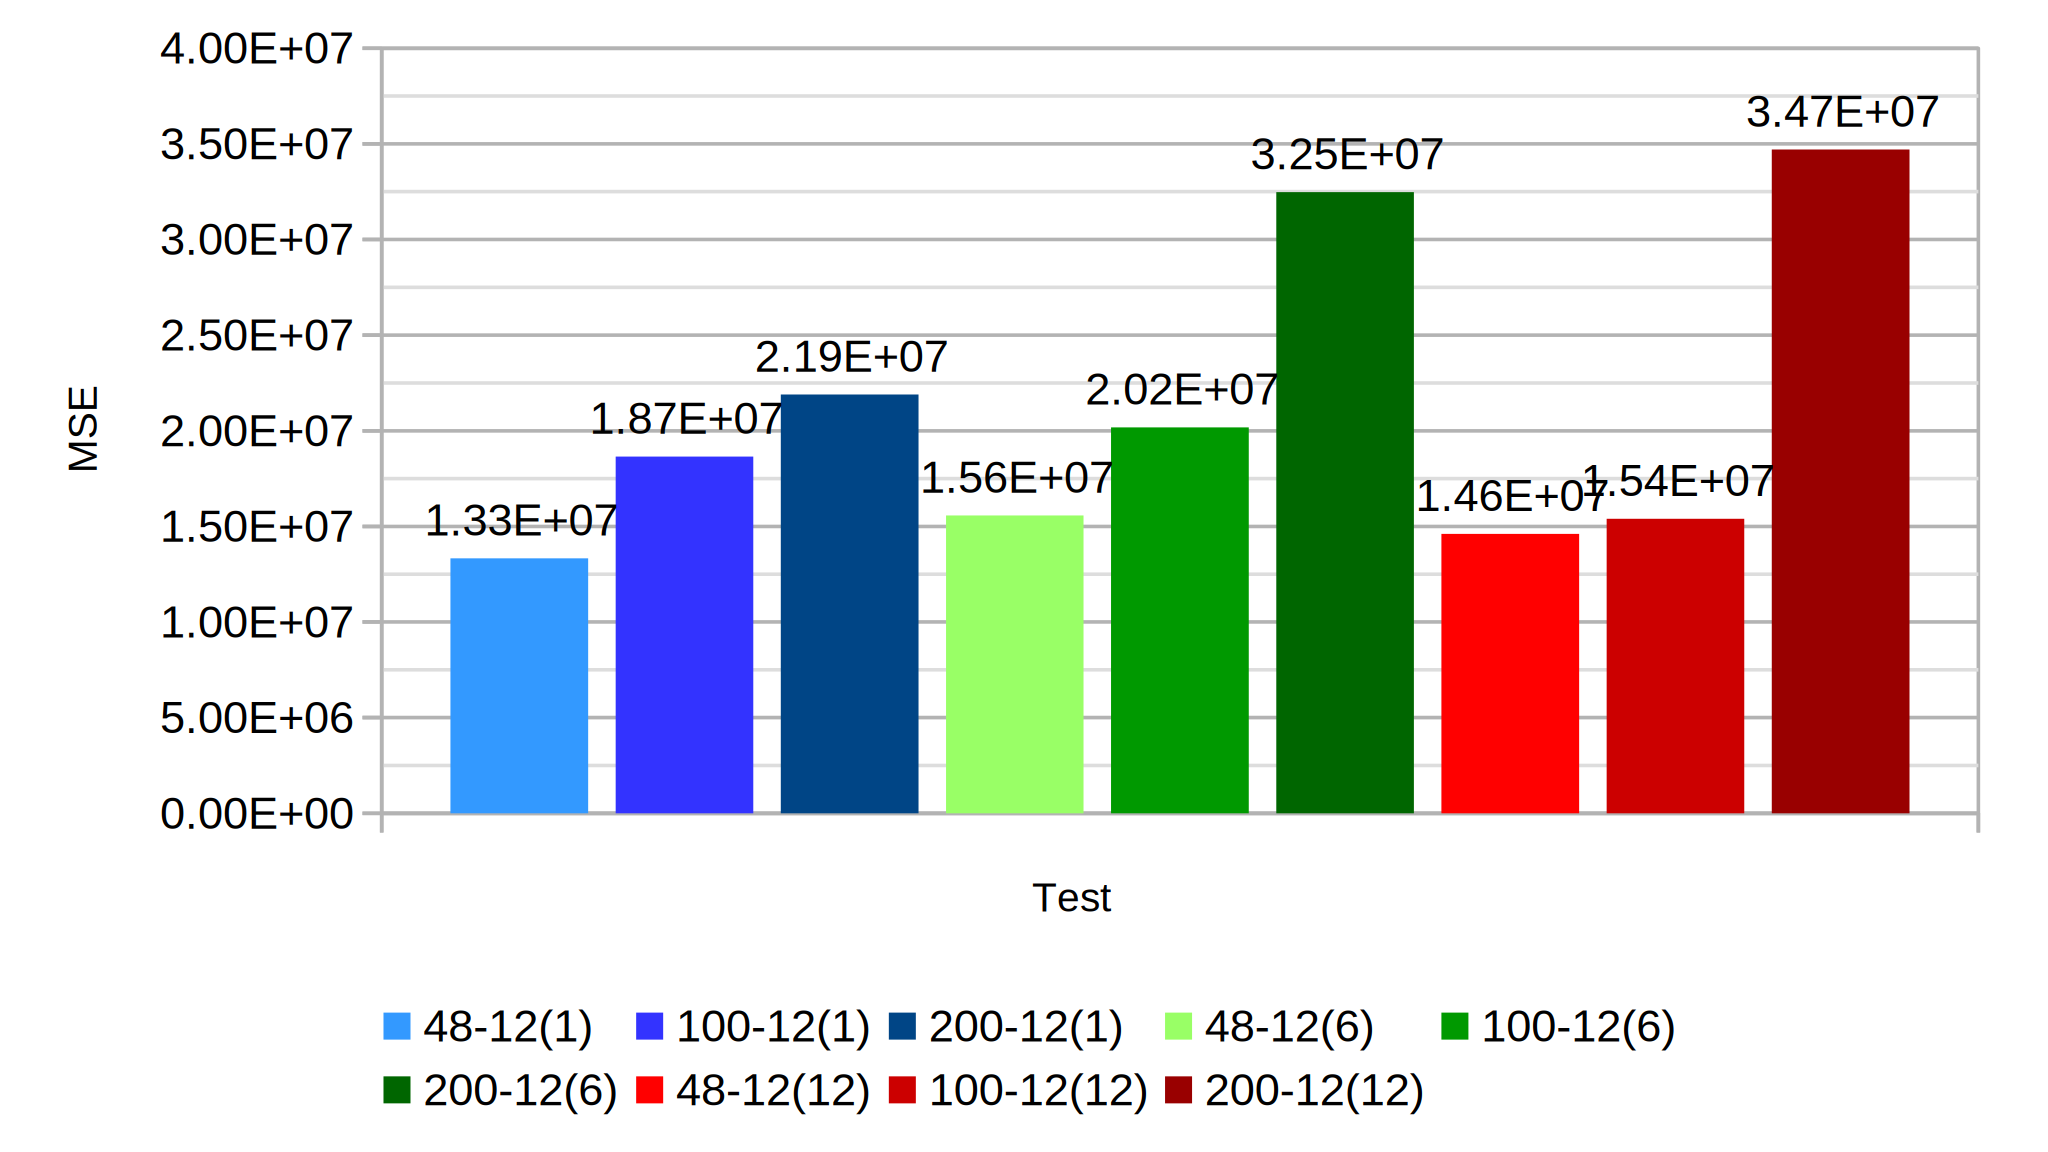
\includegraphics[angle=0]{img/src/results-double-mse.pdf}}
                \caption{Test results for double exponential smoothing. Average values of MSE for all tests samples.}
                \label{img:results-double-mse}
            \end{center}
        \end{figure}

        %%%%%%%%
        \subsection{Triple Exponential Smoothing} \label{sec:results-triple}
        Raw tests results for triple exponential smoothing are listed in Table \ref{appen:tab:triple-results}. In
        this case test cases can be run only on two data sets, because it does not make sense to fit seasonal
        model on non seasonal data. Therefore in total only eighteen tests were performed.

        During the testing it was observed that execution time of R script takes significantly more time than for other
        exponential smoothing models. On the other hand Data Mining implementation for triple exponential smoothing
        does not take more time compared to other exponential smoothing models. Table \ref{tab:datamining-perf} shows
        that R in average for one estimation takes 0.209 seconds which is for eighteen executions equals to 3.8 seconds.
        Whereas one estimation in Data Mining takes in average 0.023 seconds so time for eighteen estimation is 0.4
        seconds.

        Pie Chart \ref{img:results-triple-pie} shows that Data Mining triple exponential smoothing produces lower MSE
        in 67\% of all eighteen tests. It is better result than for simple or double exponential smoothing. However
        three tests produced MSE higher than 20\%. This could happen for example because R may use some better strategy
        for decomposing time series and setting seasonal indices.

        \begin{figure}[H]
            \begin{center}
                \begin{tikzpicture}
                    \pie[text=legend, radius=2, color={green!100 , green!50, yellow!50, red!80}]
                    {67/<1,
                    6/\interval[{1.01,1.05}],
                    6/\interval[{1.05,1.10}],
%                    11/ \interval[{1.1,1.2}],
                    22/>1.2}
                \end{tikzpicture}
                \caption{The proportion of Data Mining MSE to R MSE ratios split into intervals.}
                \label{img:results-triple-pie}
            \end{center}
        \end{figure}

        Averages of the MSE ratios are showed in Chart \ref{img:results-triple-r}. From the chart it can be seen that
        four out of nine tests produces higher MSE. R produces only 0.95 MSE in test case 200\,--\,12(12) on
        \texttt{sine} sample, but for smaller training sizes it produces 4.31 and 2.26 which is quite unstable result.
        Data Mining produces 4.07, 2.15 and 2.63 (training sets of size 50, 100 and 200). This causes significantly
        higher ratio for this test case.

        Overall results for averaged MSE ratios show that Data Mining performs better than R on smaller training sets.

        \begin{figure}[H]
            \begin{center}
                \scalebox{0.65}[0.5]{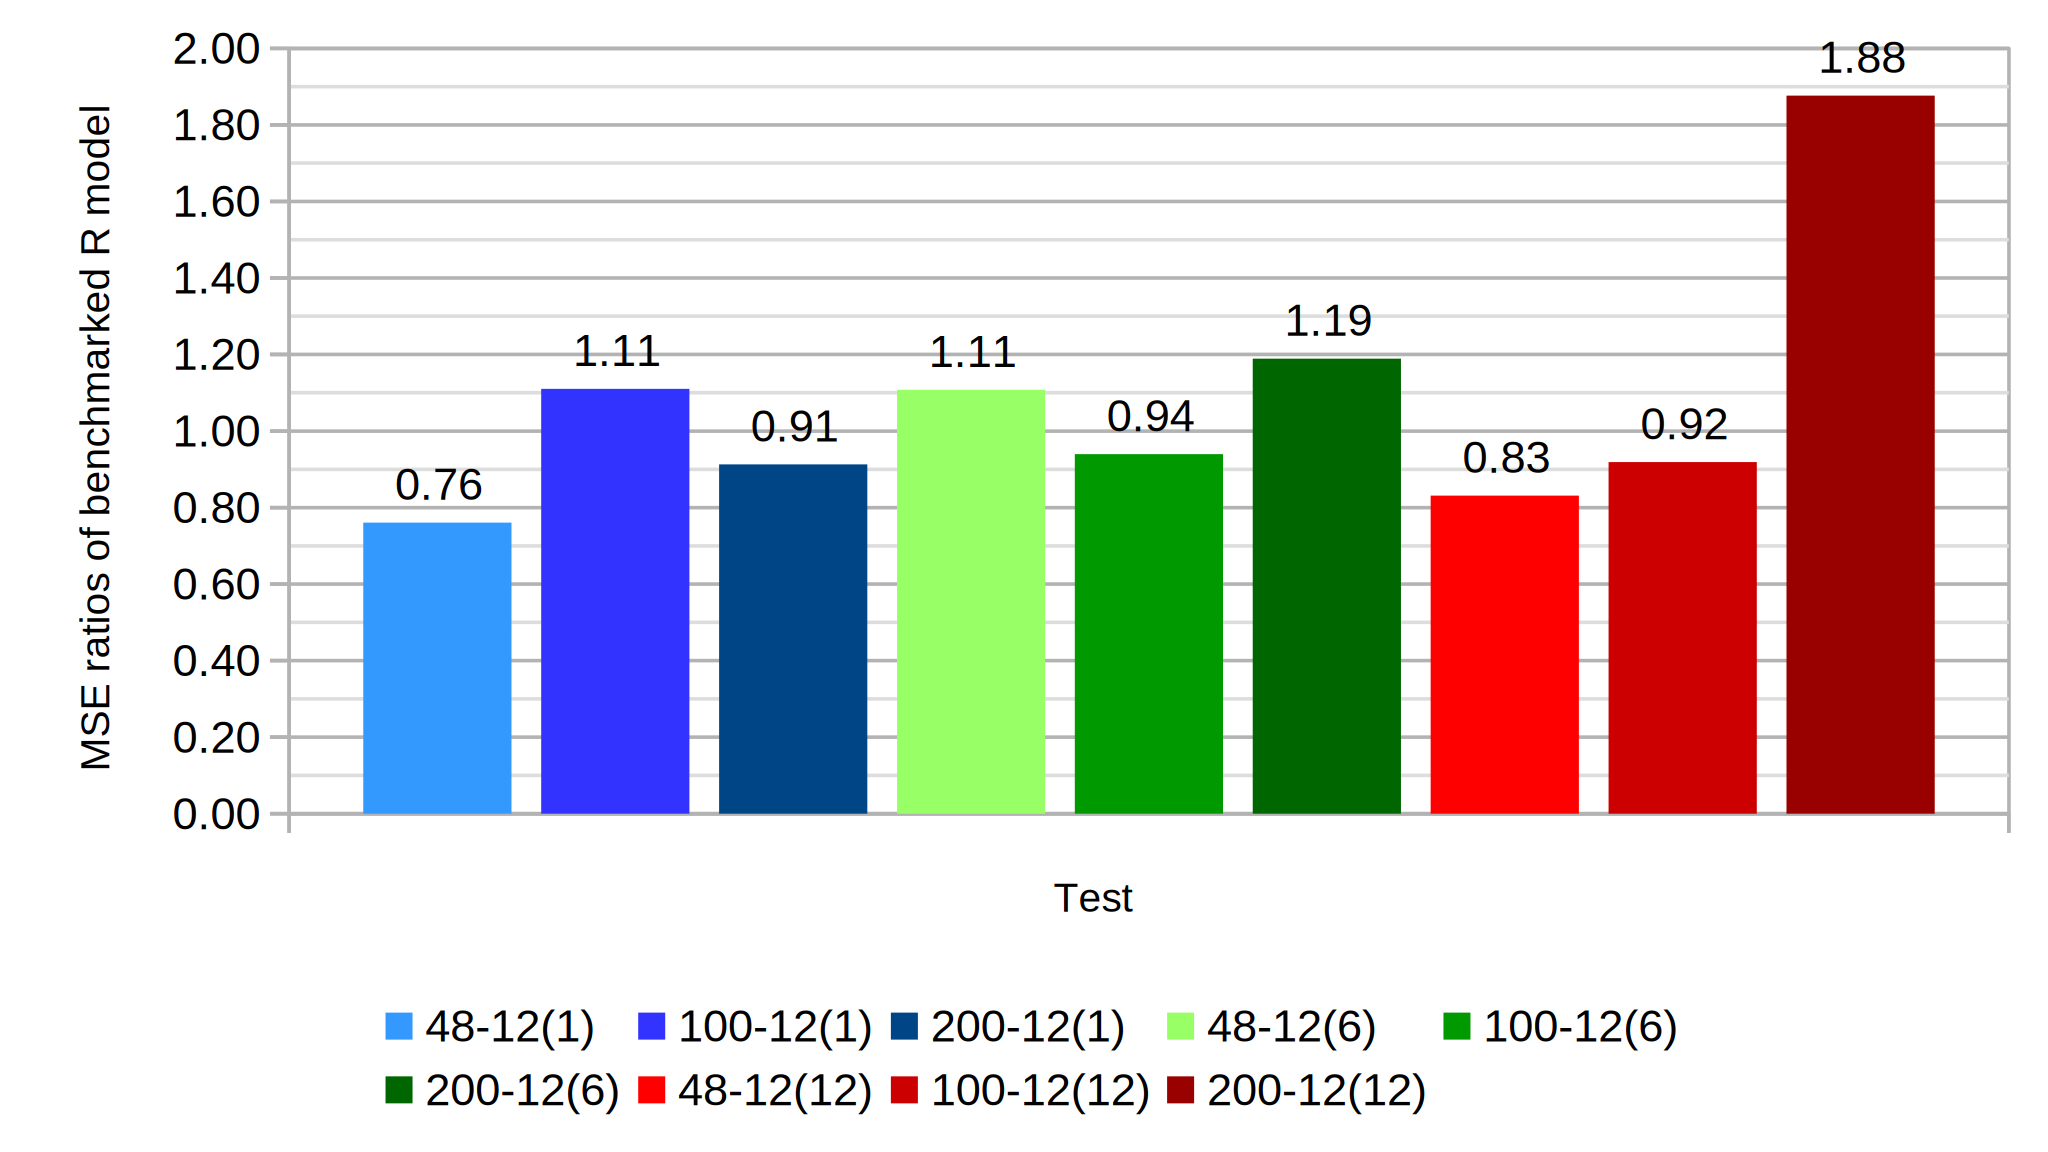
\includegraphics[angle=0]{img/src/results-triple-r.pdf}}
                \caption{Test results for triple exponential smoothing. Comparison to reference R model.}
                \label{img:results-triple-r}
            \end{center}
        \end{figure}

        Chart \ref{img:results-triple-mse} emphasize that larger training size does improve forecasting accuracy. It is
        the same result as for other models.

        \begin{figure}[H]
            \begin{center}
                \scalebox{0.65}[0.5]{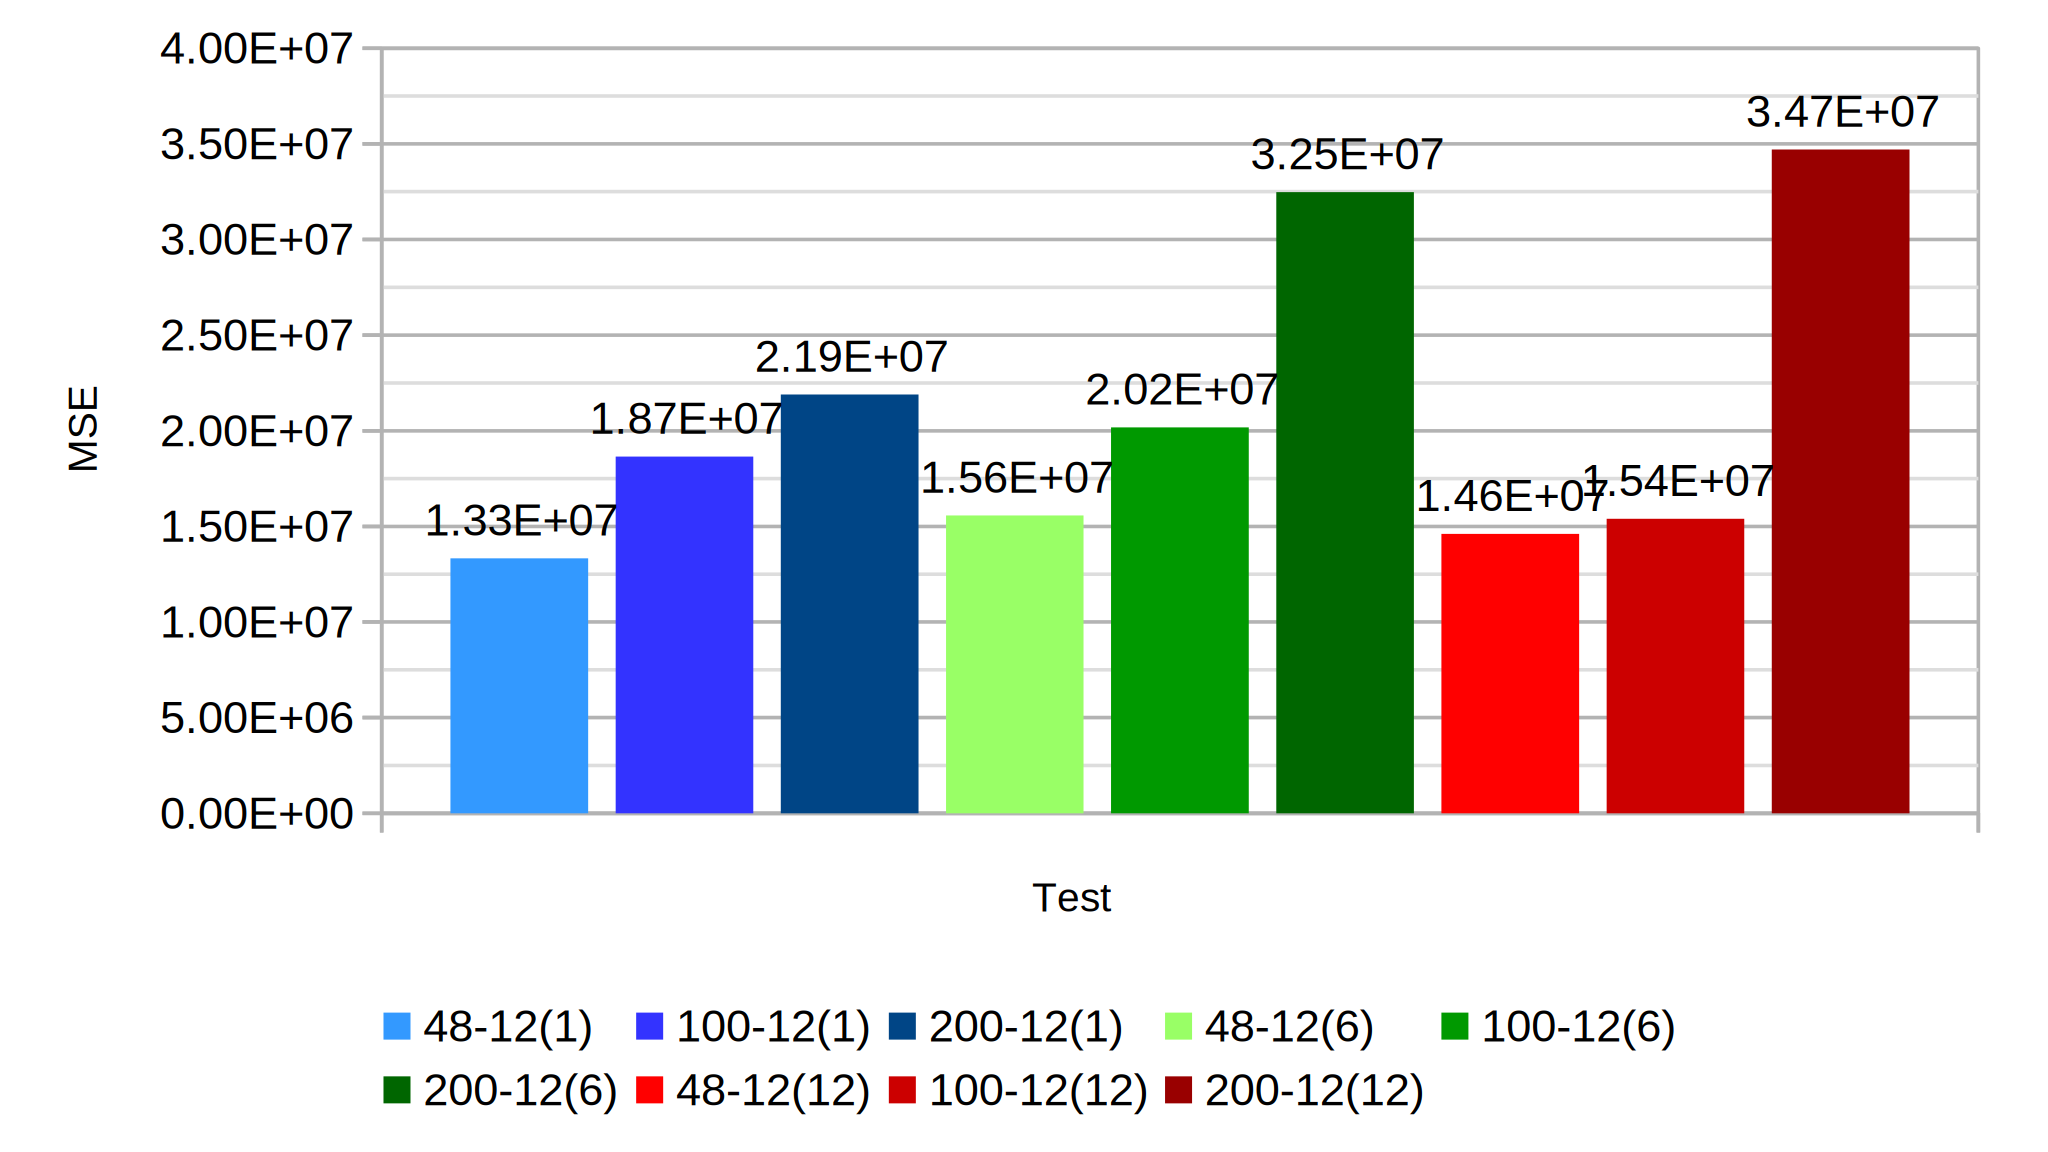
\includegraphics[angle=0]{img/src/results-double-mse.pdf}}
                \caption{Test results for triple exponential smoothing. Average values of MSE for all tests samples.}
                \label{img:results-triple-mse}
            \end{center}
        \end{figure}

        %%%%%%%%
        \subsection{Overall Results} \label{sec:overall}
        This section contains aggregated results for simple, double and triple exponential smoothing models.

        Chart \ref{img:results-overall-r} highlight that only in four tests Data Mining models in average produces
        higher MSE than alternative R models. Test case 200\,--\,12(12) shows the worst result which is 28\%
        higher than benchmarked R model. This was discussed in Section \ref{sec:results-triple}.

        Average for all test cases is equal to 2\%. In other words Data Mining models in average produced mean
        squared error higher than 2\% compared to R models. Therefore Data Mining model's prediction capabilities
        can be considered as R alternatives.

        \begin{figure}[H]
            \begin{center}
                \scalebox{0.65}[0.5]{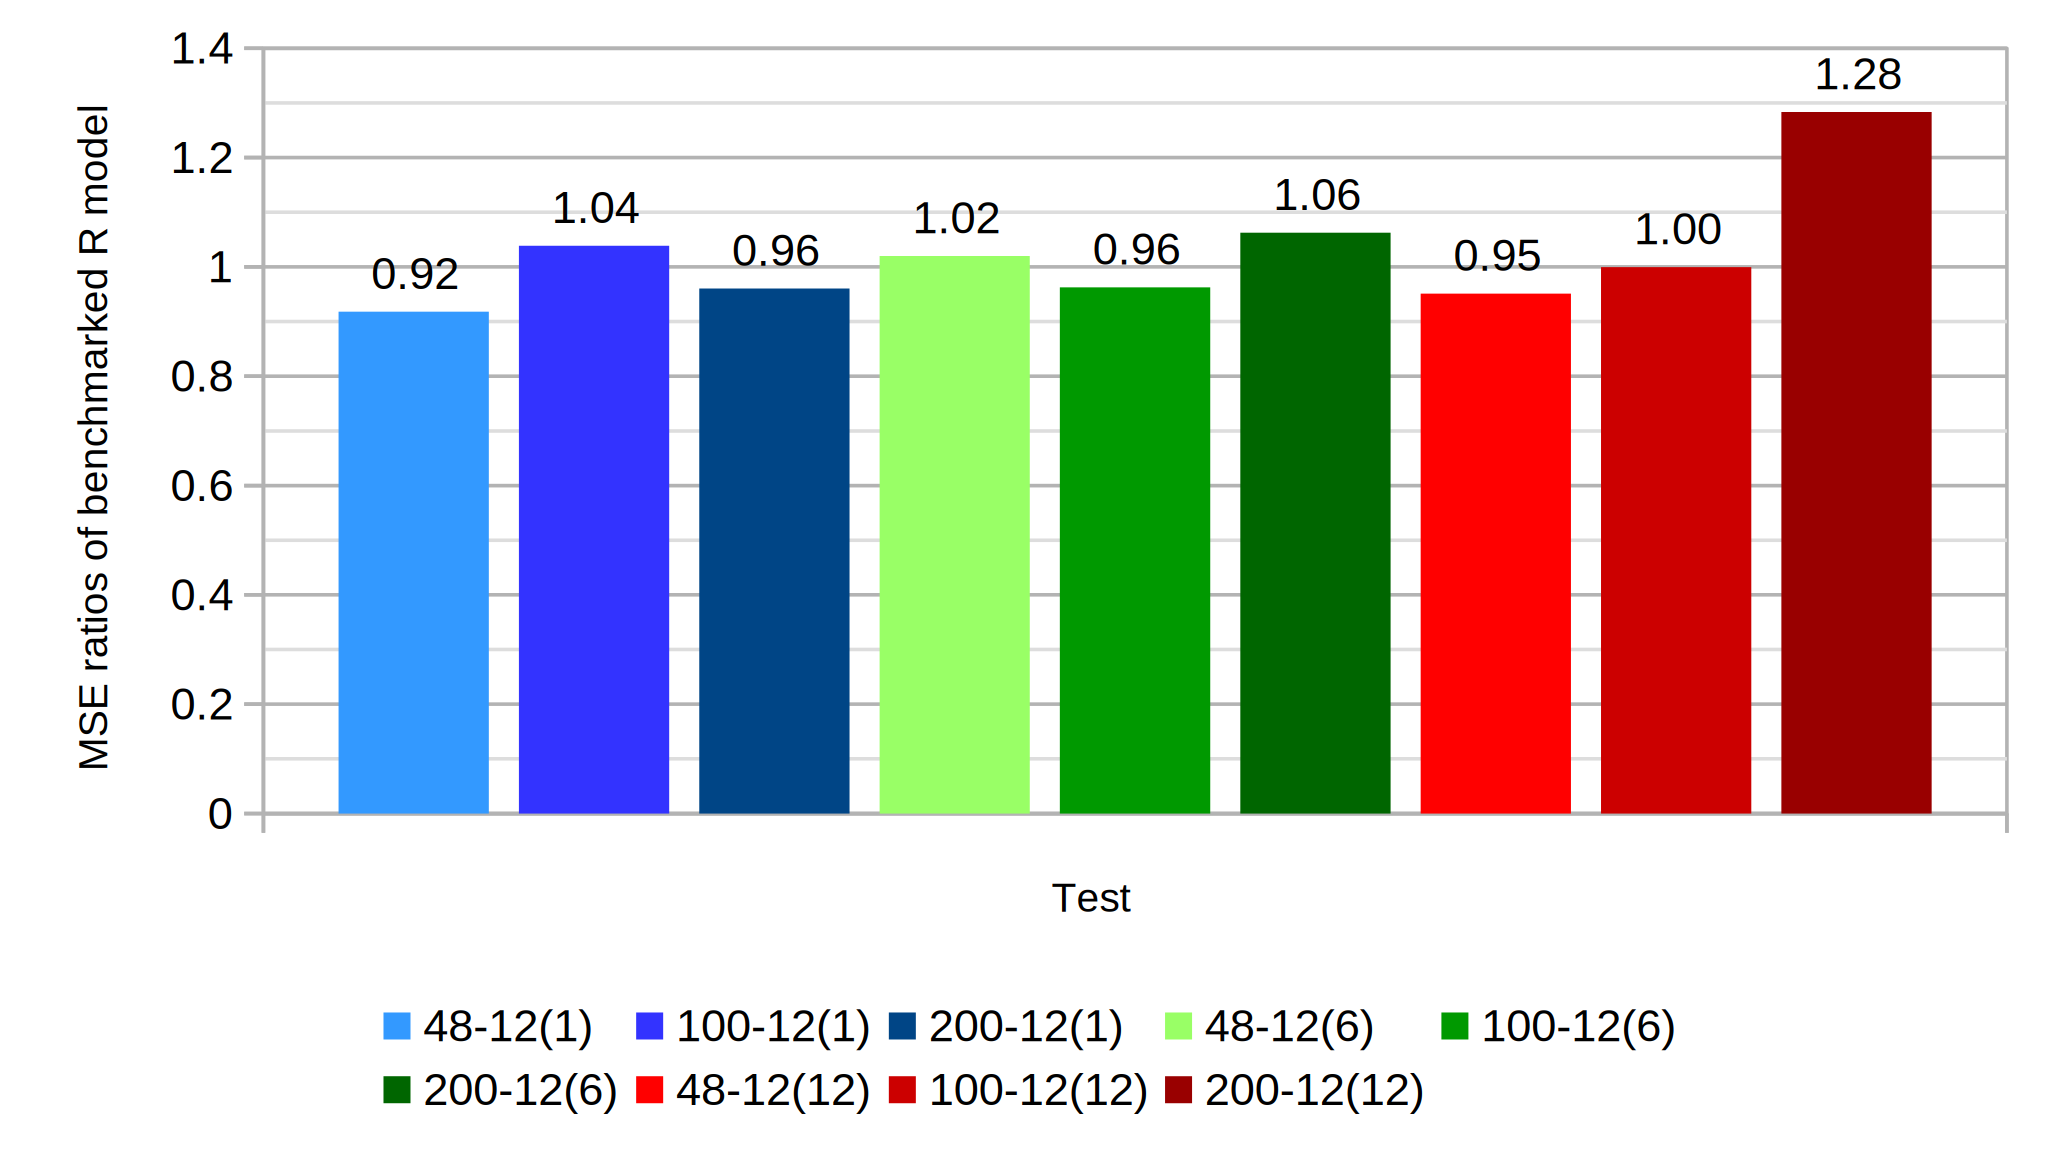
\includegraphics[angle=0]{img/src/results-overall-r.pdf}}
                \caption{Aggregated test results for all models. Comparison to reference R model.}
                \label{img:results-overall-r}
            \end{center}
        \end{figure}

        Aggregated results for Data Mining mean squared errors are depicted in Chart \ref{img:results-overall-mse}. The
        results are similar to the results discussed for each model. It shows that longer training set does not
        improve forecasting accuracy. Further research could identify ideal size of training set. These tests
        proved that longer training size does not imply better forecasts.

        \begin{figure}[H]
            \begin{center}
                \scalebox{0.65}[0.5]{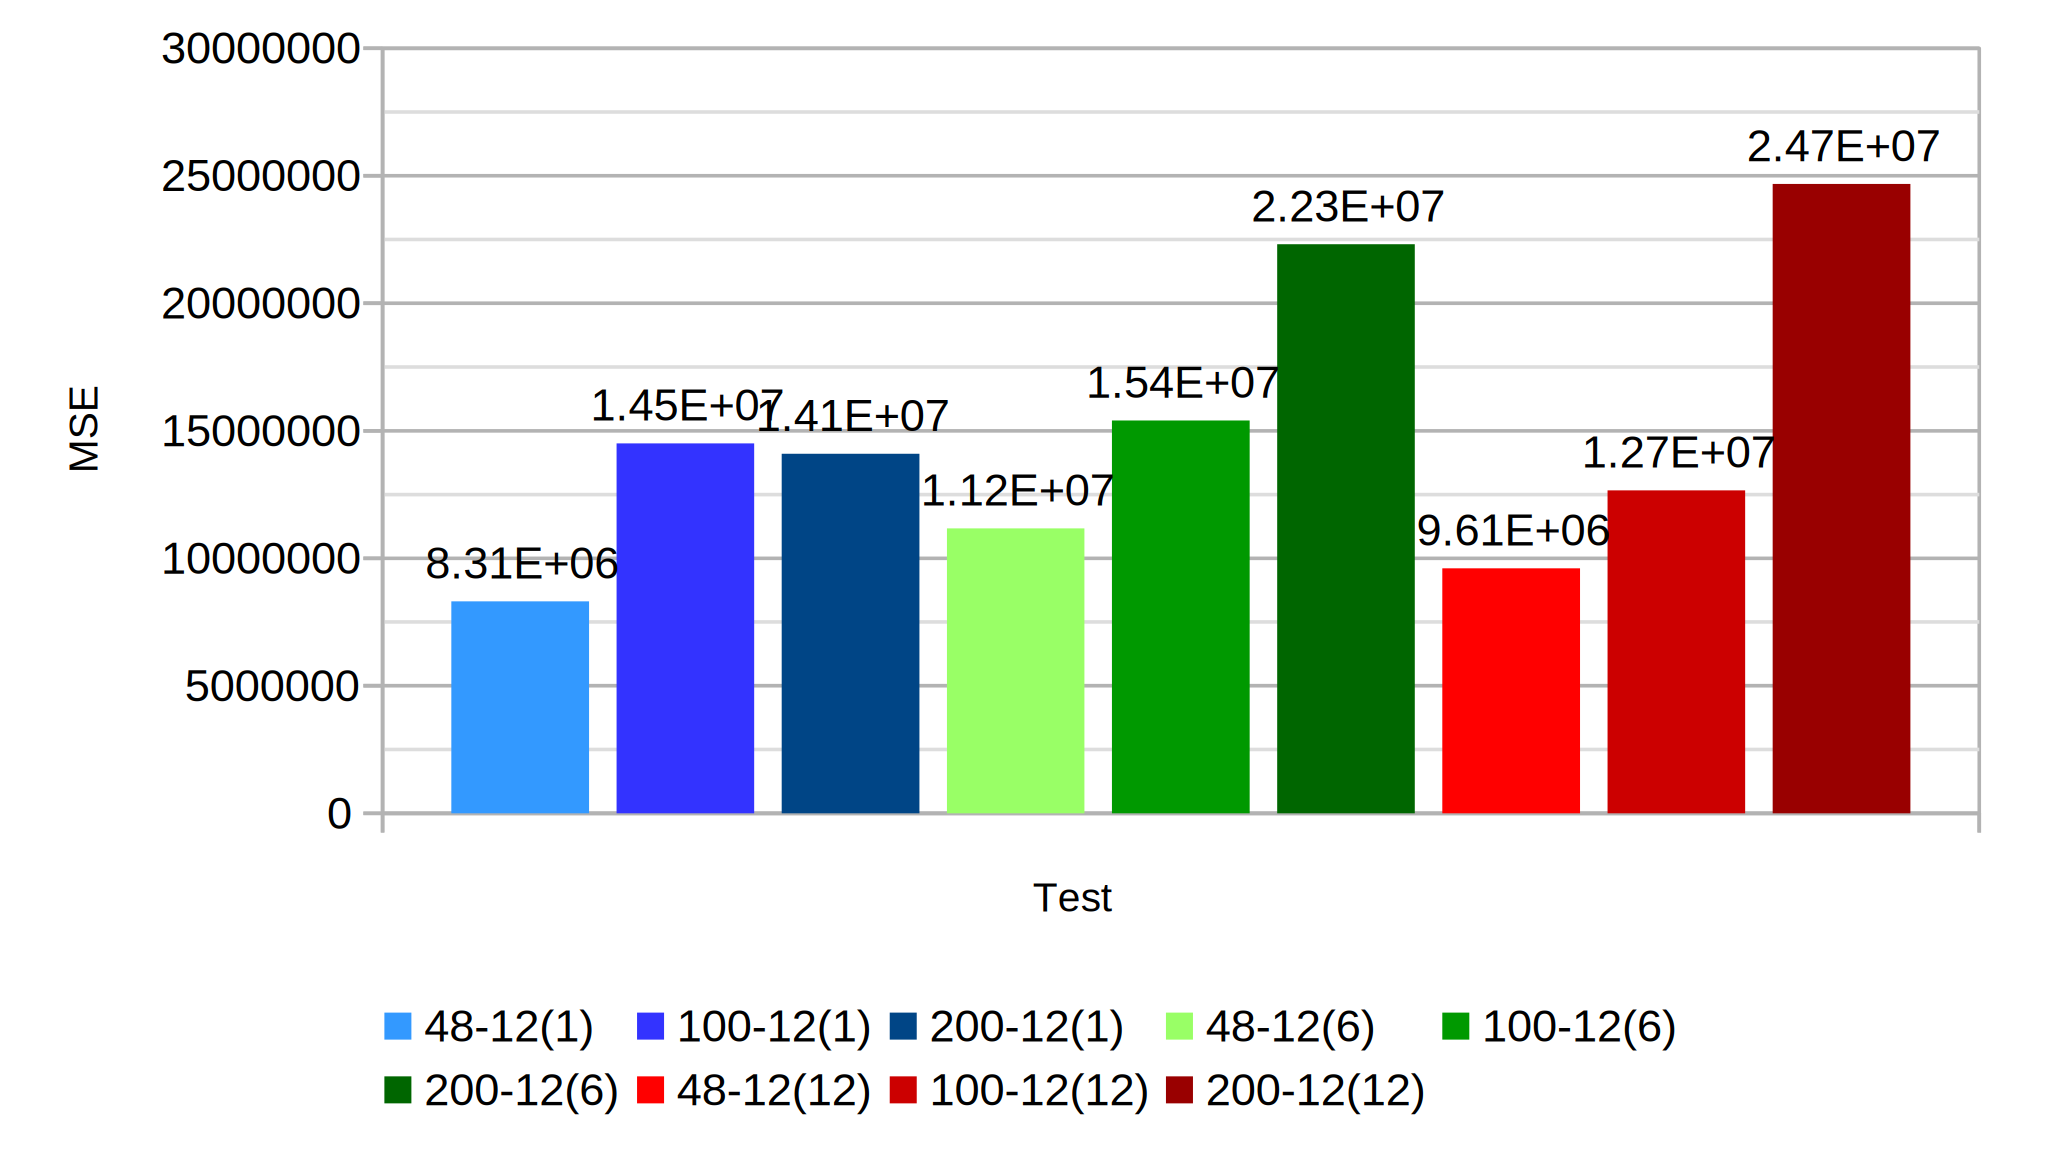
\includegraphics[angle=0]{img/src/results-overall-mse.pdf}}
                \caption{Aggregated test results for all models. Average values of MSE for all tests samples.}
                \label{img:results-overall-mse}
            \end{center}
        \end{figure}

%%%%%%%%%%%%%%%%%%%%%%%%%%%%%%%%%%%%%%%%%%%%%%%%%%%%%%%%%%%%%%%%%%%
\chapter{Conclusion} \label{chap:conclusion}
The goal of the master's thesis is to develop independent module in Java language for providing alert prediction
capabilities for open source project Hawkular.

%The thesis first describes various approaches for time series forecasting, and evaluates which methods are suitable
%for Hawkular requirements. Follows review of existing monitoring solutions and libraries for time series modelling.
%It is shown that any of existing libraries are not suitable for Hawkular, therefore a decision was made to implement
%selected models.

Implementation part is split into multiple artifacts with dedicated functionality. The most important module
focuses on time series modelling. It contains simple, double and triple exponential smoothing models which
use non-linear optimization algorithm for finding the best parameters with goal of minimizing prediction error.
The library also contains several time series utility classes and statistical tests for time series analysis.

Data Mining prediction engine autonomously selects the best time series model for underlying time series. Most
importantly, it is capable of dealing with concept drift problem. So in production there is no need of any
analytical configuration.

The last chapter benchmarks forecasting accuracy of the implemented models. It is shown that forecasts produced by
implemented models are in some cases more accurate that forecast from package \texttt{forecast} from R language and
in average Data Mining models can be compared to R models. In terms of execution time performance Data Mining
models are much efficient.

% TODO dobry cas? was?
During the development of the module, Hawkular was still in development phase, therefore it was not
possible to gather real data from production environment. This would help with tunning models for specific metrics
for example Java heap usage.

The module was successfully integrated into Hawkular and predictive charts of the metrics are located in Metric explorer
tab.

Future work on this module should analyze data from production servers and if necessary change the properties of
optimizers in order to get more accurate predictions. Analysis could also contain evaluation if damped trend should be
added to the implemented models.

As it is open source project, it would be great to attract more people into development and continue with adding new
models and features for time series analysis. Because in Java there is no widely used and maintained library.
